\section{Vortex formation at planetary gap edges in layered discs}
Gaps opened by giant planets in protoplanetary discs is a potential site for 
the RWI. Vortex formation at gap edges is seen in many 
2D and 3D hydrdynamical simulations of giant planets in low viscosity discs 
\citep{valborro07,lin10,lin11a,lin12}. The fact that this is due to the RWI has also been explicitly  
verified through linear stability analysis of planetary gap profiles 
produced from 2D simulations \citep{valborro07,lin10}. 

Here, we simulate gap-opening giant planets in 3D discs where the kinematic viscosity  
varies with height above the disc midplane. Our numerical experiments are similar
in spirit to those performed by \cite{pierens10}, but our focus here is gap stability in a 
layered disc. 

In this case the required structure for instability, the PV extremum, 
is induced by disc-planet interaction (cf. as an initial condition considered in the
previous section). We therefore initialise a 
smooth disc ($A=1$ so there is no initial bump). The associated viscous timescale
$t_\nu=r^2/\nu\sim 10^3P_0$ (for $\hat{\nu}\sim 10^{-4}$) is much
longer than our simulation timescale. It is not crucial to initialize
the simulation with an exact steady state since the giant planet
maintains the gap. We therefore employ a simpler viscosity profile than
the previous experiment.   
%no initial pert

\subsection{Viscosity profile}\label{planet_visc_mode}
Using the same notation as \S\ref{visc_model}, we impose a viscosity
profile $\hat{\nu}$ such that 
\begin{align}\label{planet_visc_profile}
  \hat{\nu}\Sigma_i(R)\frac{d\ln{\Omega_i}}{d\ln{R}} =
  \hat{\nu}_0\left[1+Q(\psi)\right]\Sigma_i(r_0)\left.\frac{d\ln{\Omega_i}}{d\ln{R}}\right|_{r_0}.      
\end{align}
We have set the dimensionless argument in Eq. \ref{step} to
$\zeta=\psi$. The viscosity increases by a factor $A_\nu$ for 
$\psi > \zeta_\nu$. So the viscous layer is 
a wedge in the meridional plane, which conveniently fits into our
spherical grid. Fig. \ref{planet_visc2d} gives an example of this
viscosity profile. We will quote the thickness of the viscous layer as a 
percentage of the entire $\theta$ domain size. 

\begin{figure}
  \centering
  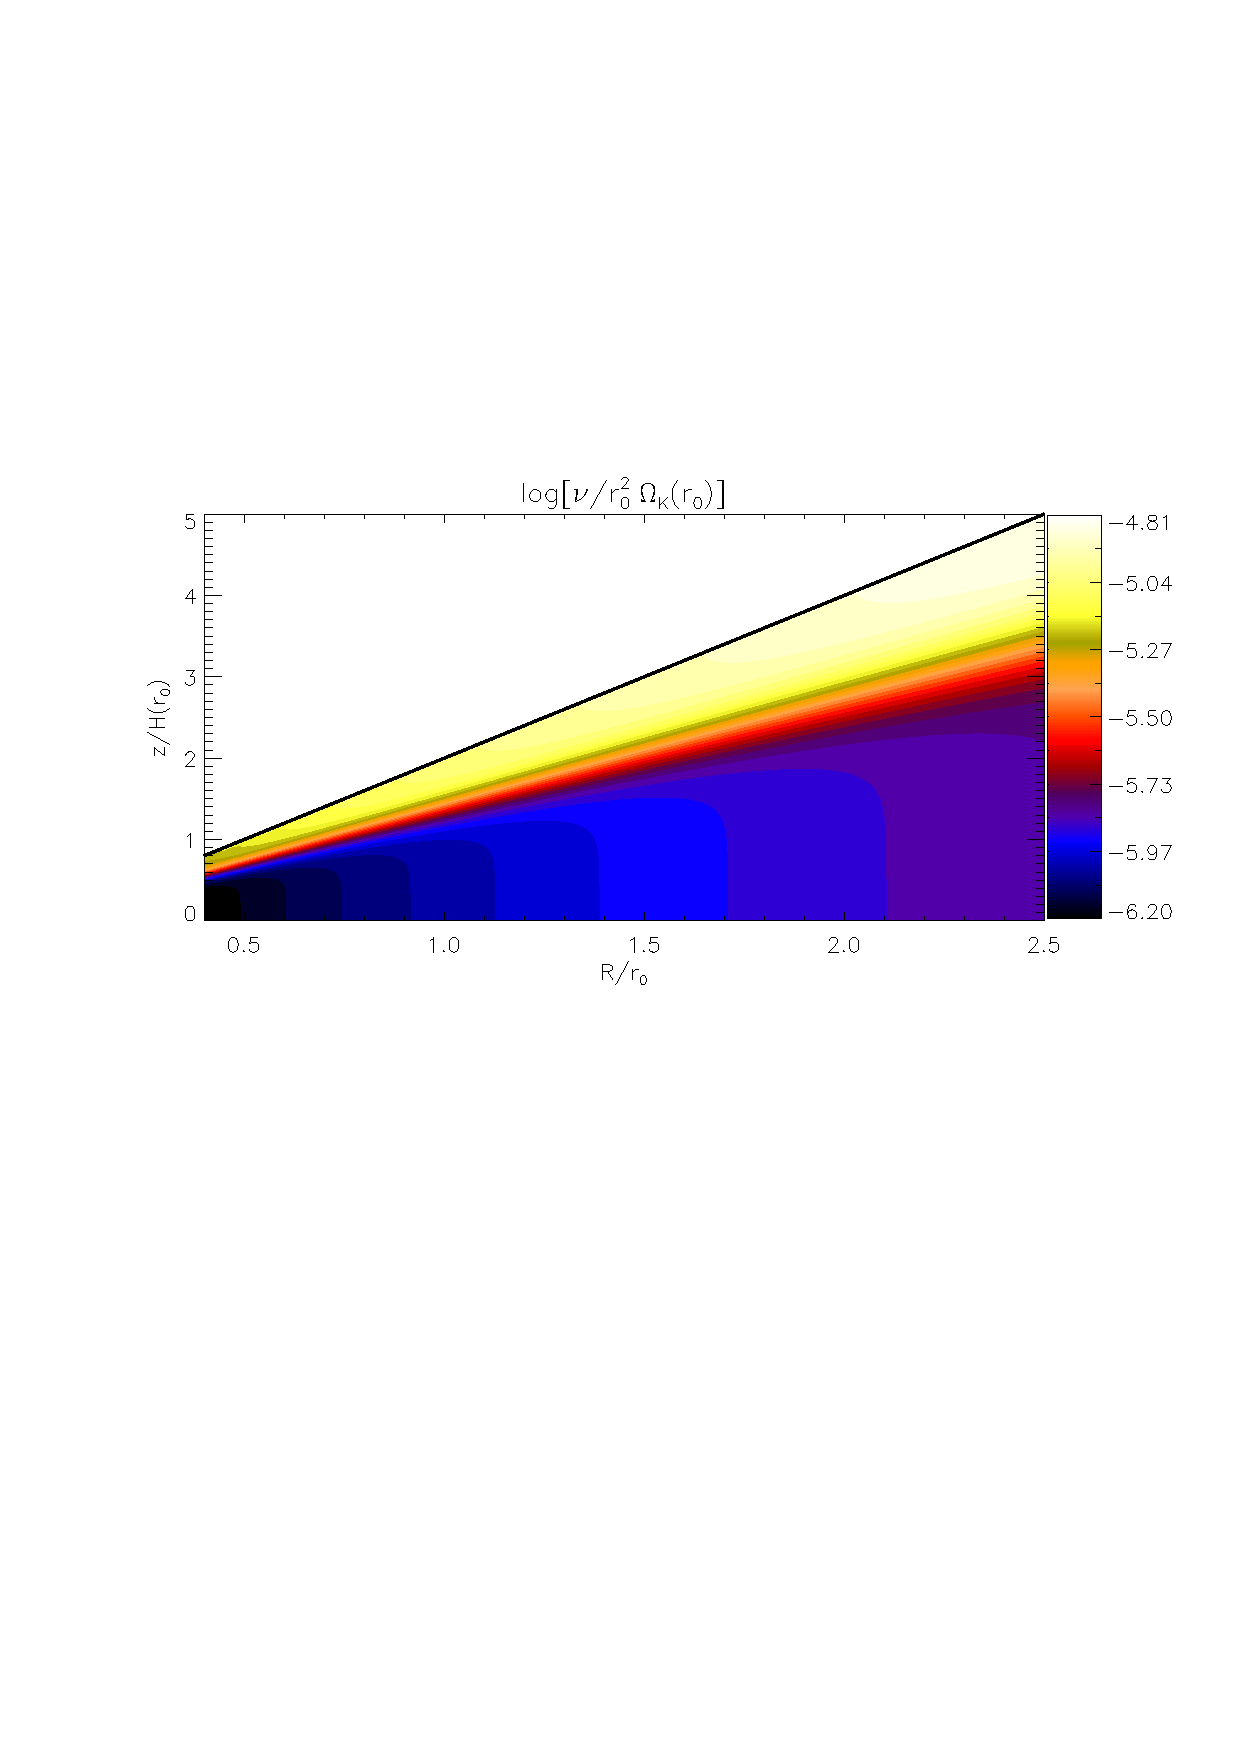
\includegraphics[width=\linewidth]{figures/pdisk_visc2d_planet}
  \caption{Example of the `wedge' viscosity profile
    imposed in disc-planet simulations (Eq. \ref{planet_visc_profile}). This specific plot
    corresponds to case P1. The solid line
    delineates the upper boundary of the computational domain.
    \label{planet_visc2d}}
\end{figure}

We set the floor viscosity $\hat{\nu}_0=10^{-6}$. The more typical
value adopted for disc-planet simulations, $\hat{\nu}_0\sim 10^{-5}$,
is known to surpress vortex formation in 2D simulations
\citep{valborro07, mudryk09}. The angluar thickness of the viscosity
transition is fixed to $\Delta\zeta_\nu = 0.2h$.   

Note that setting $\psi = 0$ in Eq. \ref{planet_visc_profile} gives
the appropriate viscosity profile for a razor-thin viscous disc in
steady state when the initial cylindrical radial velocity 
is set by Eq. \ref{init_vr}. 

\subsection{Disc-planet simulations} 
We simulate discs with $h=0.05$ and radial extent
$[\rin,\rout]=[0.4,2.5]r_0$. The initial cylindrical radial velocity
is given by Eq. \ref{init_vr}. The standard resolution is $(N_r,
N_\theta, N_\phi)=(256, 32n_h, 768)$, corresponding to $6,\,32,\,6$
cells per $H$ along the $r,\theta,\phi$ directions 
at the reference radius. 

We use a planetary mass 
$M_p=10^{-3}M_*$, which corresponds to a Jupiter mass planet if
$M_*=M_{\sun}$. The softening length adopted for the planet potential is
$\epsilon_p=0.5r_h$. The planet potential is switched on 
smoothly over $t\in[0,10]P_0$. We note that the disc can be considered
as two-dimensional for gap-opening giant planets, because the Hill
radius $r_h$ exceeds the local scale-height $H_0$ ($r_h/H_0\simeq1.4$
in our cases).   

We remark that the above choice of physical and numerical parameter
values are typical for global disc-planet simulations
\citep[e.g.][]{valborro06,mignone12}.  


\subsubsection{Standard runs} 
The fiducial vertical extent of our disc model is $n_h=2$
scale-heights at $R=r_0$.  The control run, case P0, has $A_\nu=1$ so there is 
no viscous layer. The kinematic viscosity is therefore
$\hat{\nu}\sim10^{-6}$  everywhere. We then introduce a viscous
layer (or wedge) occupying the uppermost $25\%$ and $50\%$ of the
vertical domain in cases P1 and P2, by choosing the transition angle
at $\zeta_\nu = 1.5h,\,1.0h$, respectively. These layers have a kinematic 
viscosity of $\hat{\nu}\sim 10^{-5}$ by setting $A_\nu=10$.  (See
Fig. \ref{planet_visc2d} for the viscosity profile for case P1.)  

For completeness we also performed two high-viscosity simluations
which do not develop vortices. Case P3 has $\hat{\nu}\sim10^{-5}$
throughout the vertical extent, while in case P4 the uppermost $25\%$
of the vertical domain has $\hat{\nu}\sim10^{-4}$. The purpose is to
examine how a stable gap profile is affected by layered viscosity. 

\subsubsection{Extended vertical domain}
We also consider two runs with an extended vertical domain size
$n_h=3$. Case P5 has $A_\nu=1$ so there is no viscous layer. For case
P6 we set the transition angle $\zeta_\nu=2h$ with $A_\nu=100$. 
Thus, the viscous layer with $\hat{\nu}\sim10^{-4}$ occupies $33\%$ of
the uppermost vertical domain. 
%We also consider case P6 without a
%viscous layer but 


%%%%%%%%%%%%%%%%%%%%%%%%%%%%%%%%%%%%%%%%%%%%%%%%%%%%%%%%%%%%%%%%%%%%%%%%%%%%%%%


\subsection{Results}
Our disc-planet simulations are summarised in Table \ref{planet_sims}.
We focus on vortex-formation at the outer gap edge. 
The non-axisymmetric mode amplitude in the last column was 
averaged over the shell $r\in[1.2,1.6]r_0$ and over time 
$t\in[100,150]P_0$. We examine the $m=1$ mode since 
for non-self-gravitating planetary gaps, if unstable, usually develop
a single vortex in quasi-steady state \citep{valborro07,lin10}.   

%for  mode amp: spatial average over [1.2,1.6], time average over [100,150]P_0

\begin{table}
  \centering
  \caption{Summary of disc-planet simulations. These runs employ the
    `wedge' viscosity model described by
    Eq. \ref{planet_visc_profile}. The upper viscous layer is
    quoted as a fraction of the vertical domain at 
    $R=r_0$. \label{planet_sims}}  
    \begin{tabular}{lccccr}
      \hline\hline
      %      \multicolumn{6}{c}{\phantom{stuff}} &
      %      \multicolumn{3}{c}{Linear phase ($t\leq10P_0$)}&
      %      \multicolumn{3}{c}{$t=100P_0$}\\
      %      \cline{7-9}\cline{10-12}
      Case & $n_h$ & $A_\nu$ &$\zeta_\nu/h$ & visc. layer& $10^2\overline{a}_1$ \\ 
      \hline
      P0 &  2     &    1    &    n/a      & none     &   14.3    \\% Ro~ -0.03
      P1 &  2     &    10   &    1.5      & $25\%$  &    11.9     \\ 
      P2 &  2     &    10   &    1.0      & $50\%$  &    6.1      \\
      P3 &  2     &    10   &    n/a      & none    &    ??      \\
      P4&  2     &    100  &    1.5      & $25\%$  &    ??     \\
      P5 &  3     &    1    &     n/a      & none  &     18.3   \\
      P6 &  3     &    100   &    2.0      & $33\%$ &     3.5    \\
%      P6 &  3     &    100   &    n/a      & none   &     ??     \\
      \hline
  \end{tabular}
\end{table}

\subsection{Thickening the viscous layer}
We first compare cases P0, P1 and P2. Fig. \ref{planet_gap} 
shows that the PV profiles induced by the planet is very
similar. (In fact, case P0 and P1 already non-axisymmetric
disturbances at the chosen snapshot, but they are weak and is not
reflected in the azimuthally averaged PV plots.) This shows that gap
opening is not sensitive to the presence of a viscous layer.  

\begin{figure}
  \centering
  \includegraphics[width=\linewidth]{figures/pdisk_vorten1d_cases_002.ps}
  \caption{Potential vorticity perturbation in the disc-planet
    simulations P0, P1 and P2. The snapshot is taken 10 orbits after
    the planet is fully introduced. %% Both P0 and P1 already developed
    %% small non-axisymmetric
    \label{planet_gap}}
\end{figure}

Indeed, the density perturbations shown for $t=50P_0$ in
Fig. \ref{jup0} indicates that the RWI develops in all cases. This is
consistent with our previous experiments which show that the linear
instability is largely unaffected by viscous layers. However,   
the $t=50P_0$ snapshot shows that thickening the viscous layer does lead
to somewhat larger vortices, as expected because of viscous diffusion.   

However, a viscous layer can have significant influences  
well into the non-linear regime. Fig. \ref{jup0} shows that the vortex
merging proceeds in case P0 to form a single vortex at the outer gap
edge at $t=100P_0$. This is a standard result for giant planets in
low viscosity discs \citep{valborro06,valborro07}.  

The final vortex is weaker 
in case P1, as indicated by the $m=1$ amplitude in Table
\ref{planet_sims}. Most interestingly, the vortices are transient in case P2,
being absent after $t=100P_0$. This means that vortex formation can be
surpressed by viscous layers. This suggests that for long-term vortex
survival, the entire vertical extent of the disc should be `dead'. 

\begin{figure}
   \centering
   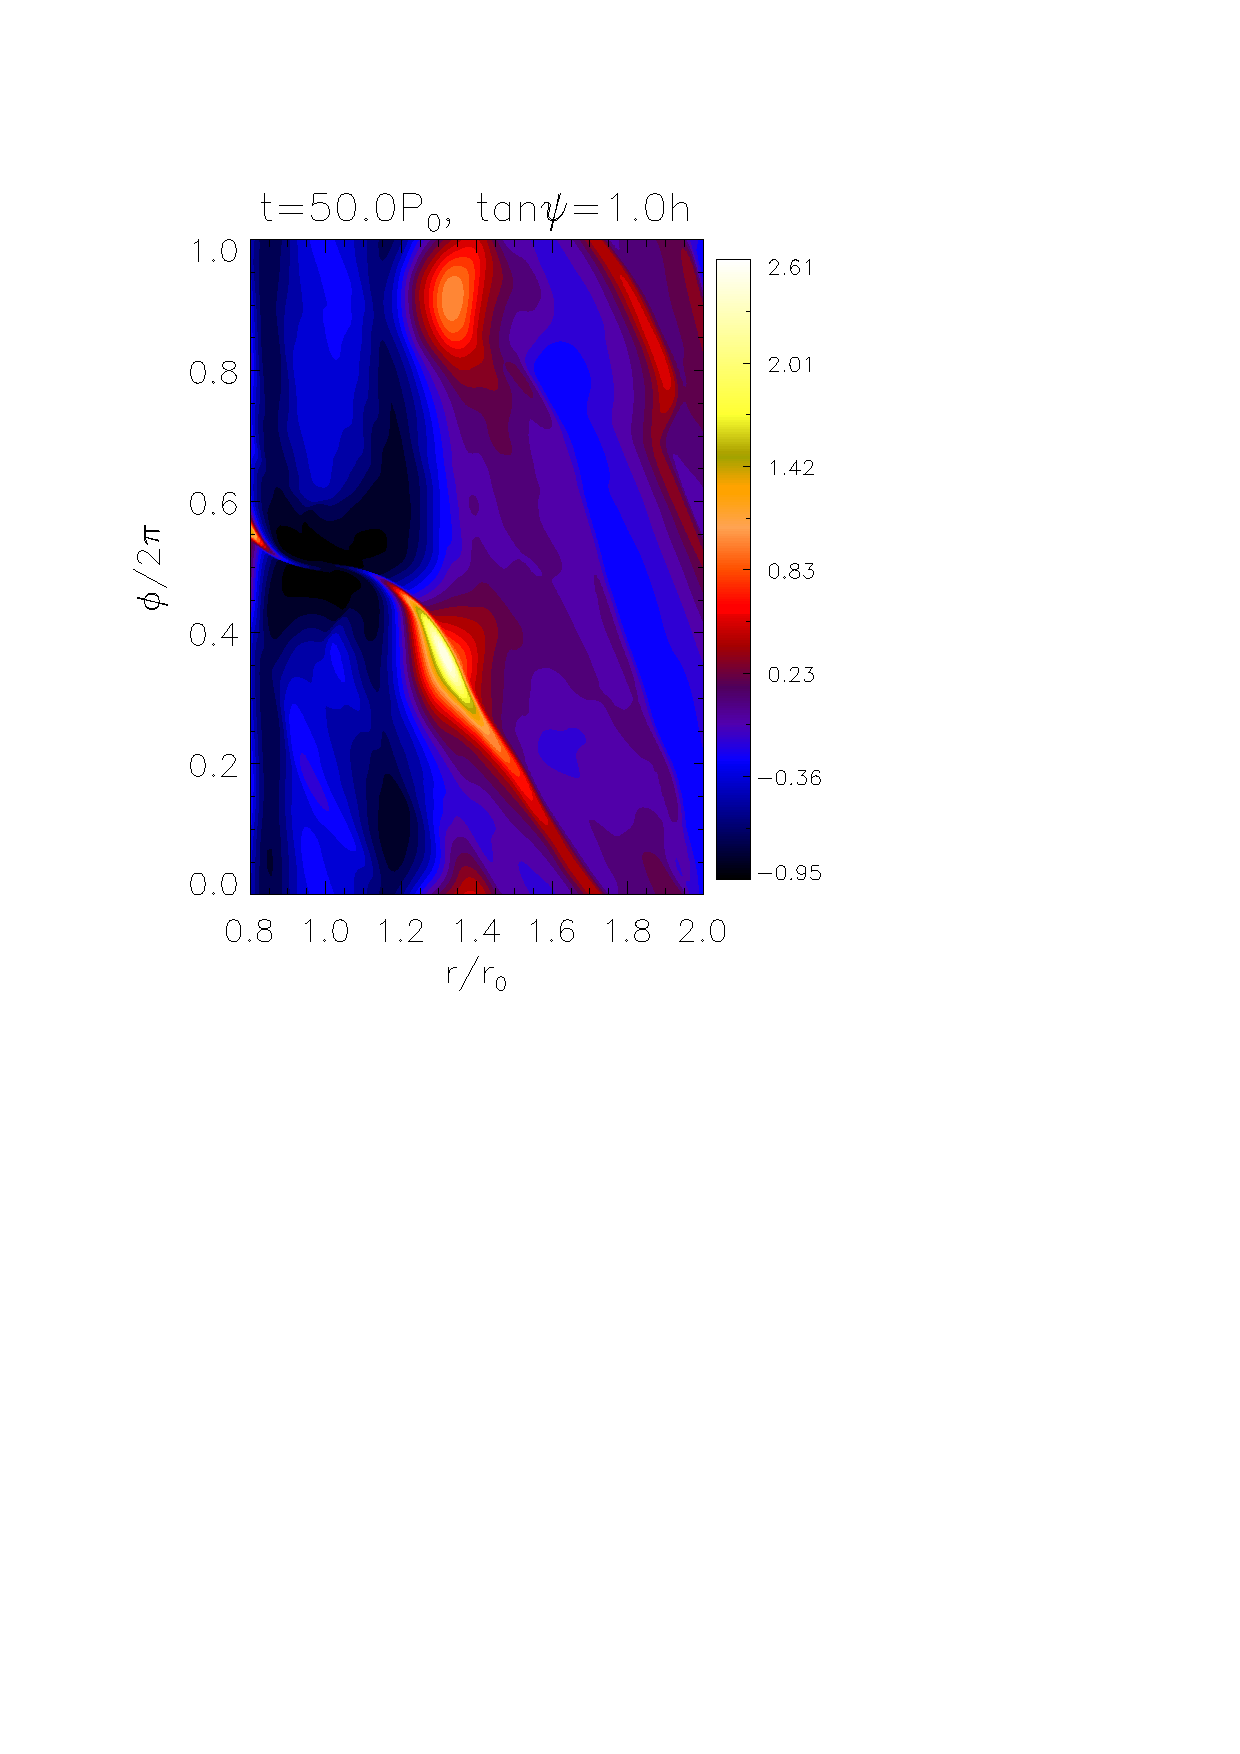
\includegraphics[scale=.39,clip=true,trim=0cm 1.84cm 0cm
     0cm]{figures/jup0_pdisk005}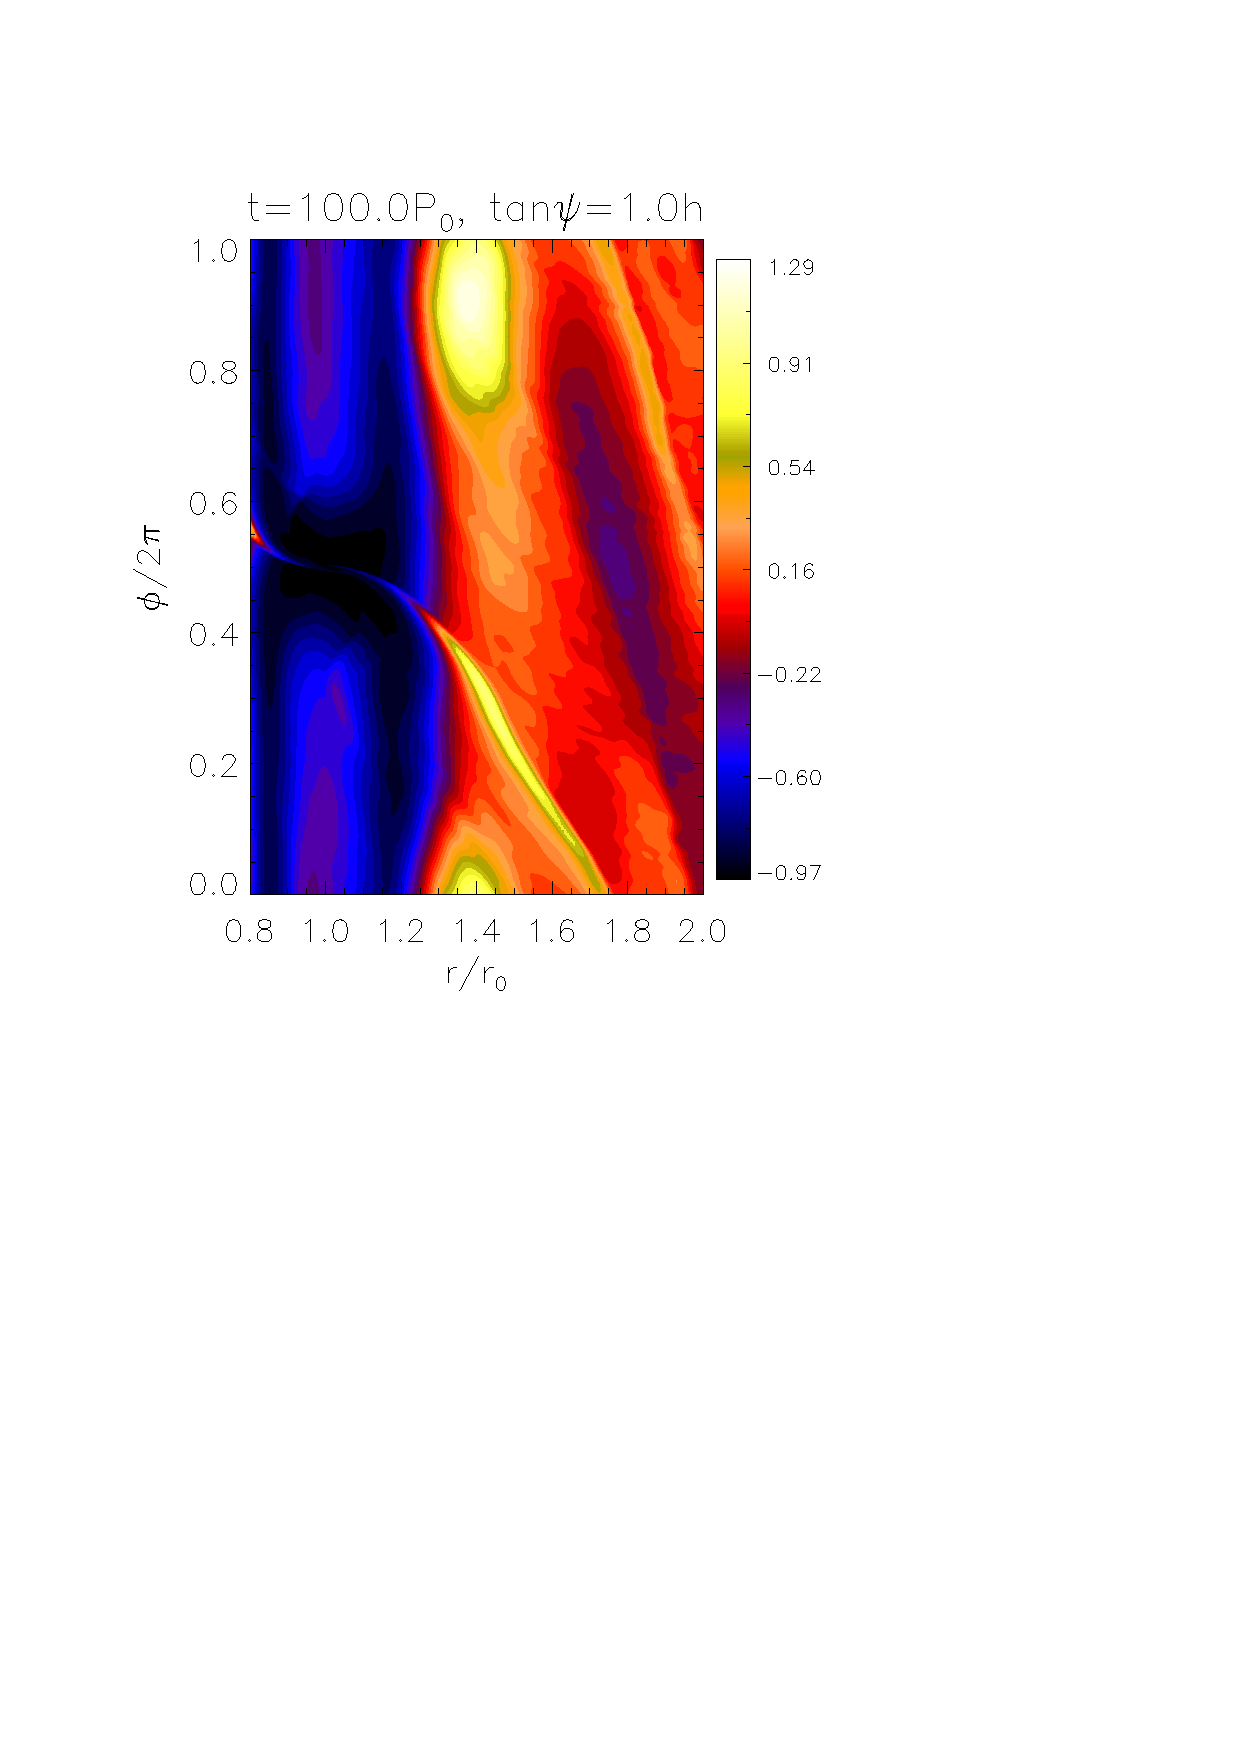
\includegraphics[scale=.39,clip=true,trim=2.3cm
     1.84cm 0cm
     0cm]{figures/jup0_pdisk010}\\%% 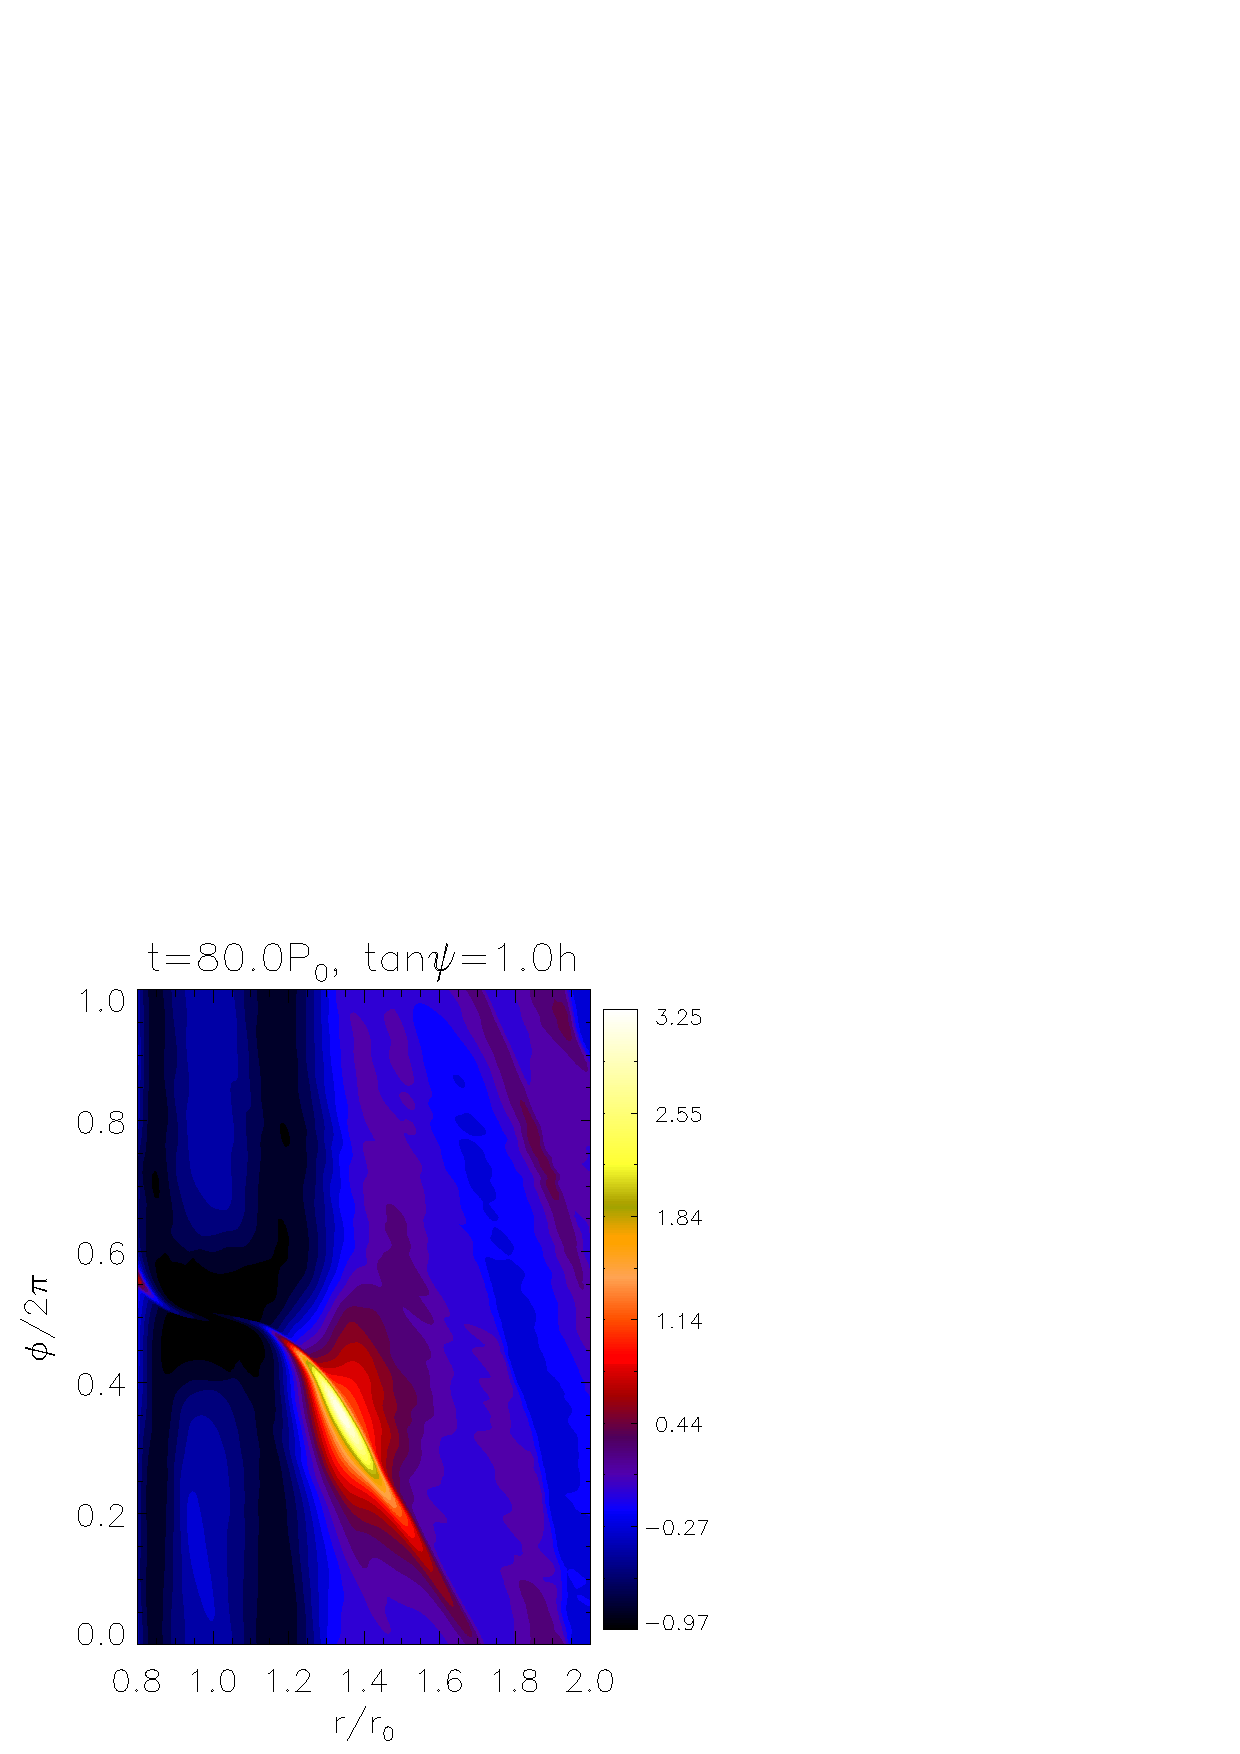
\includegraphics[scale=.27,clip=true,trim=2.3cm
     %% 1.84cm 0cm
     %% 0cm]{figures/jup0_pdisk008}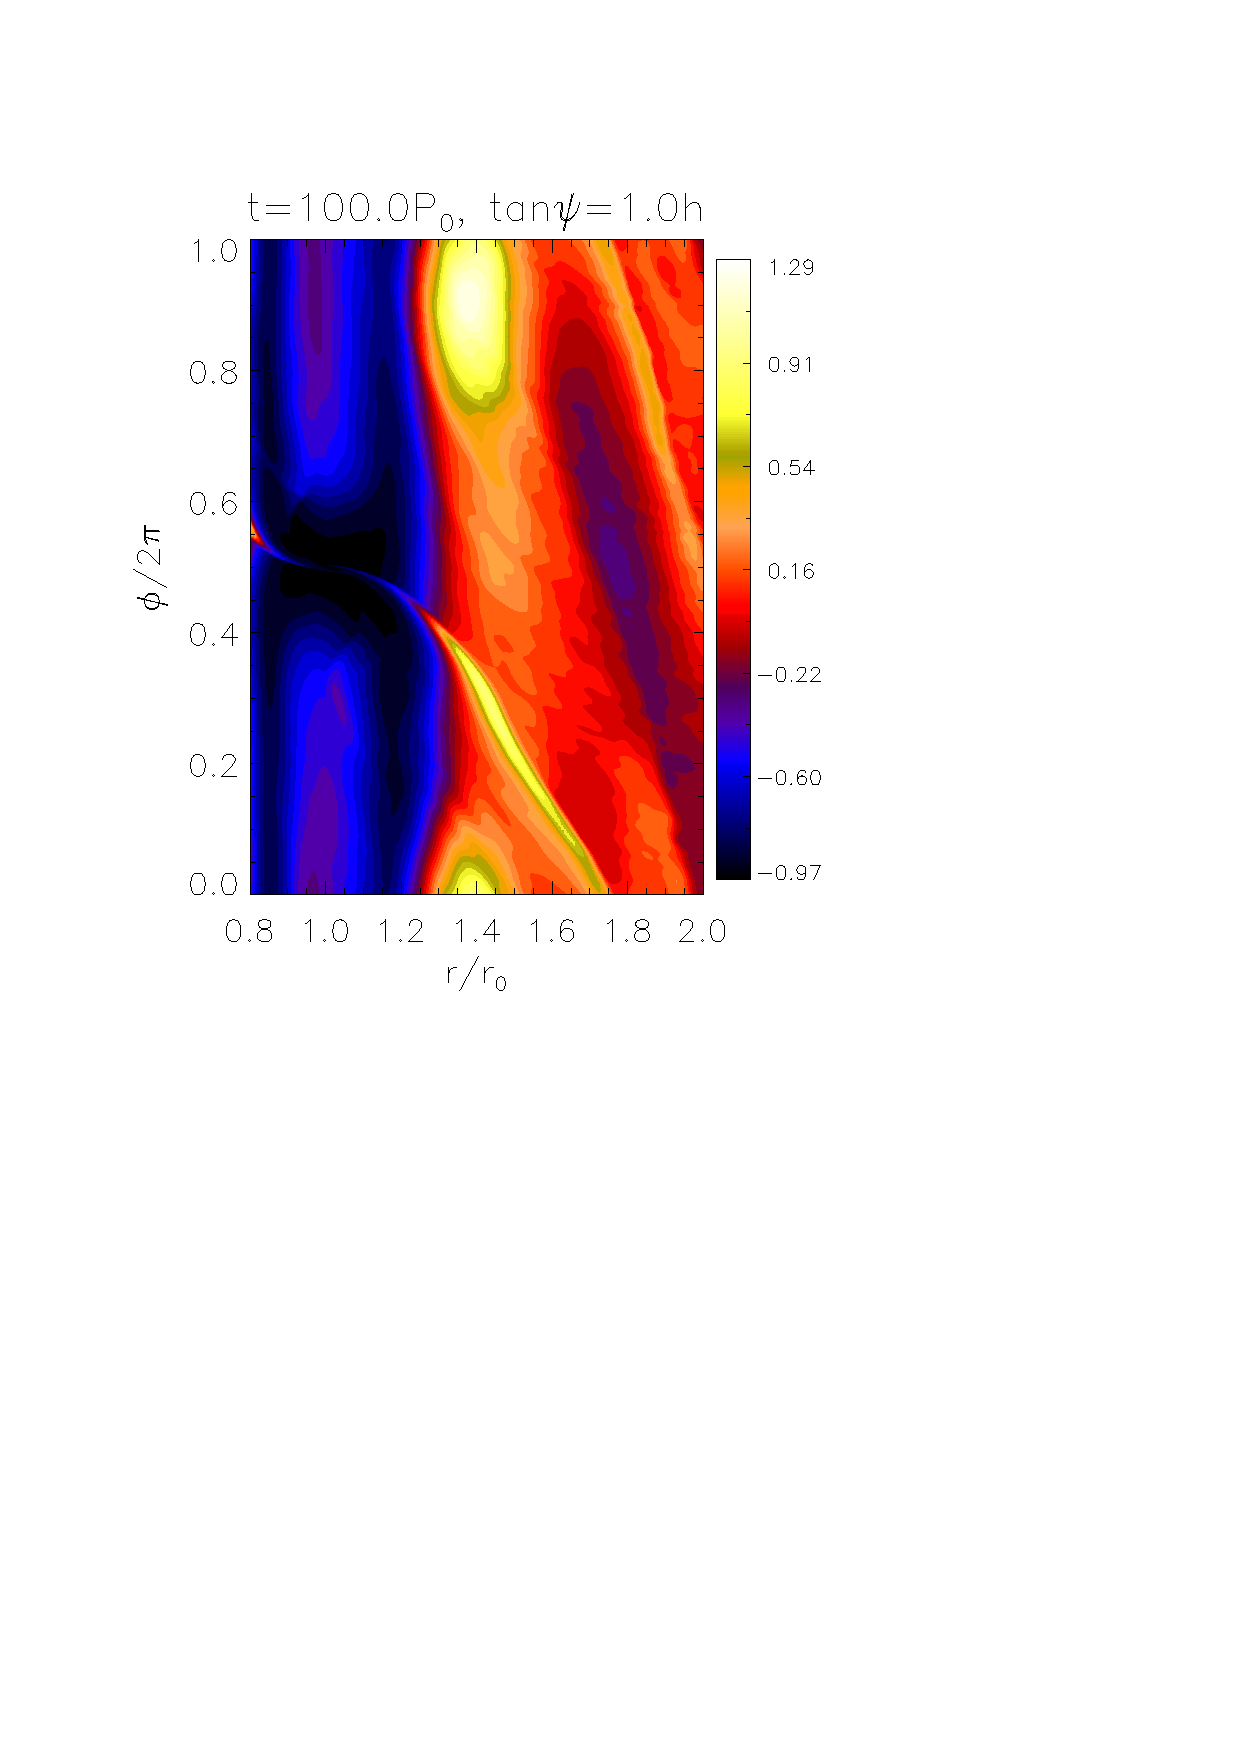
\includegraphics[scale=.27,clip=true,trim=2.3cm
     %% 1.84cm 0cm
     %% 0cm]{figures/jup0_pdisk010}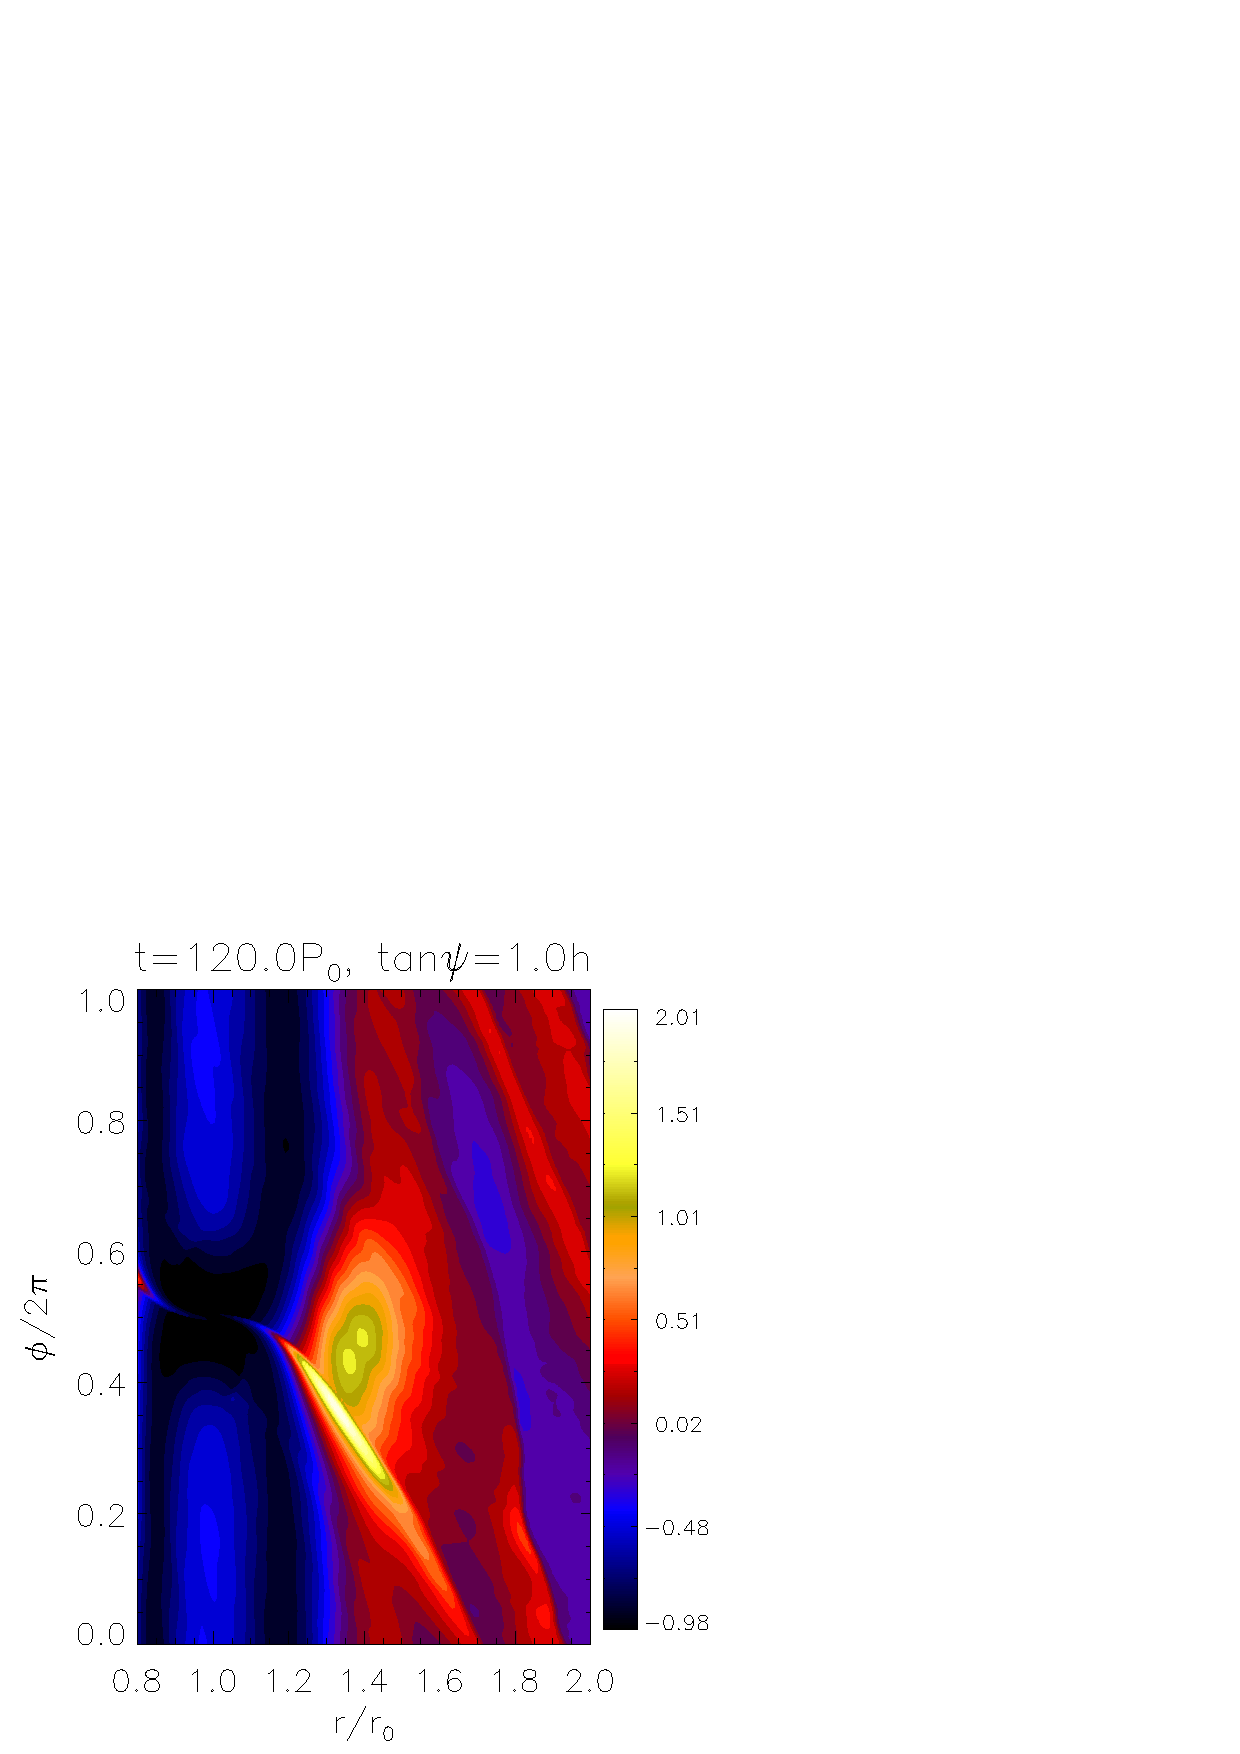
\includegraphics[scale=.27,clip=true,trim=2.3cm
     %% 1.84cm 0cm
     %% 0cm]{figures/jup0_pdisk012}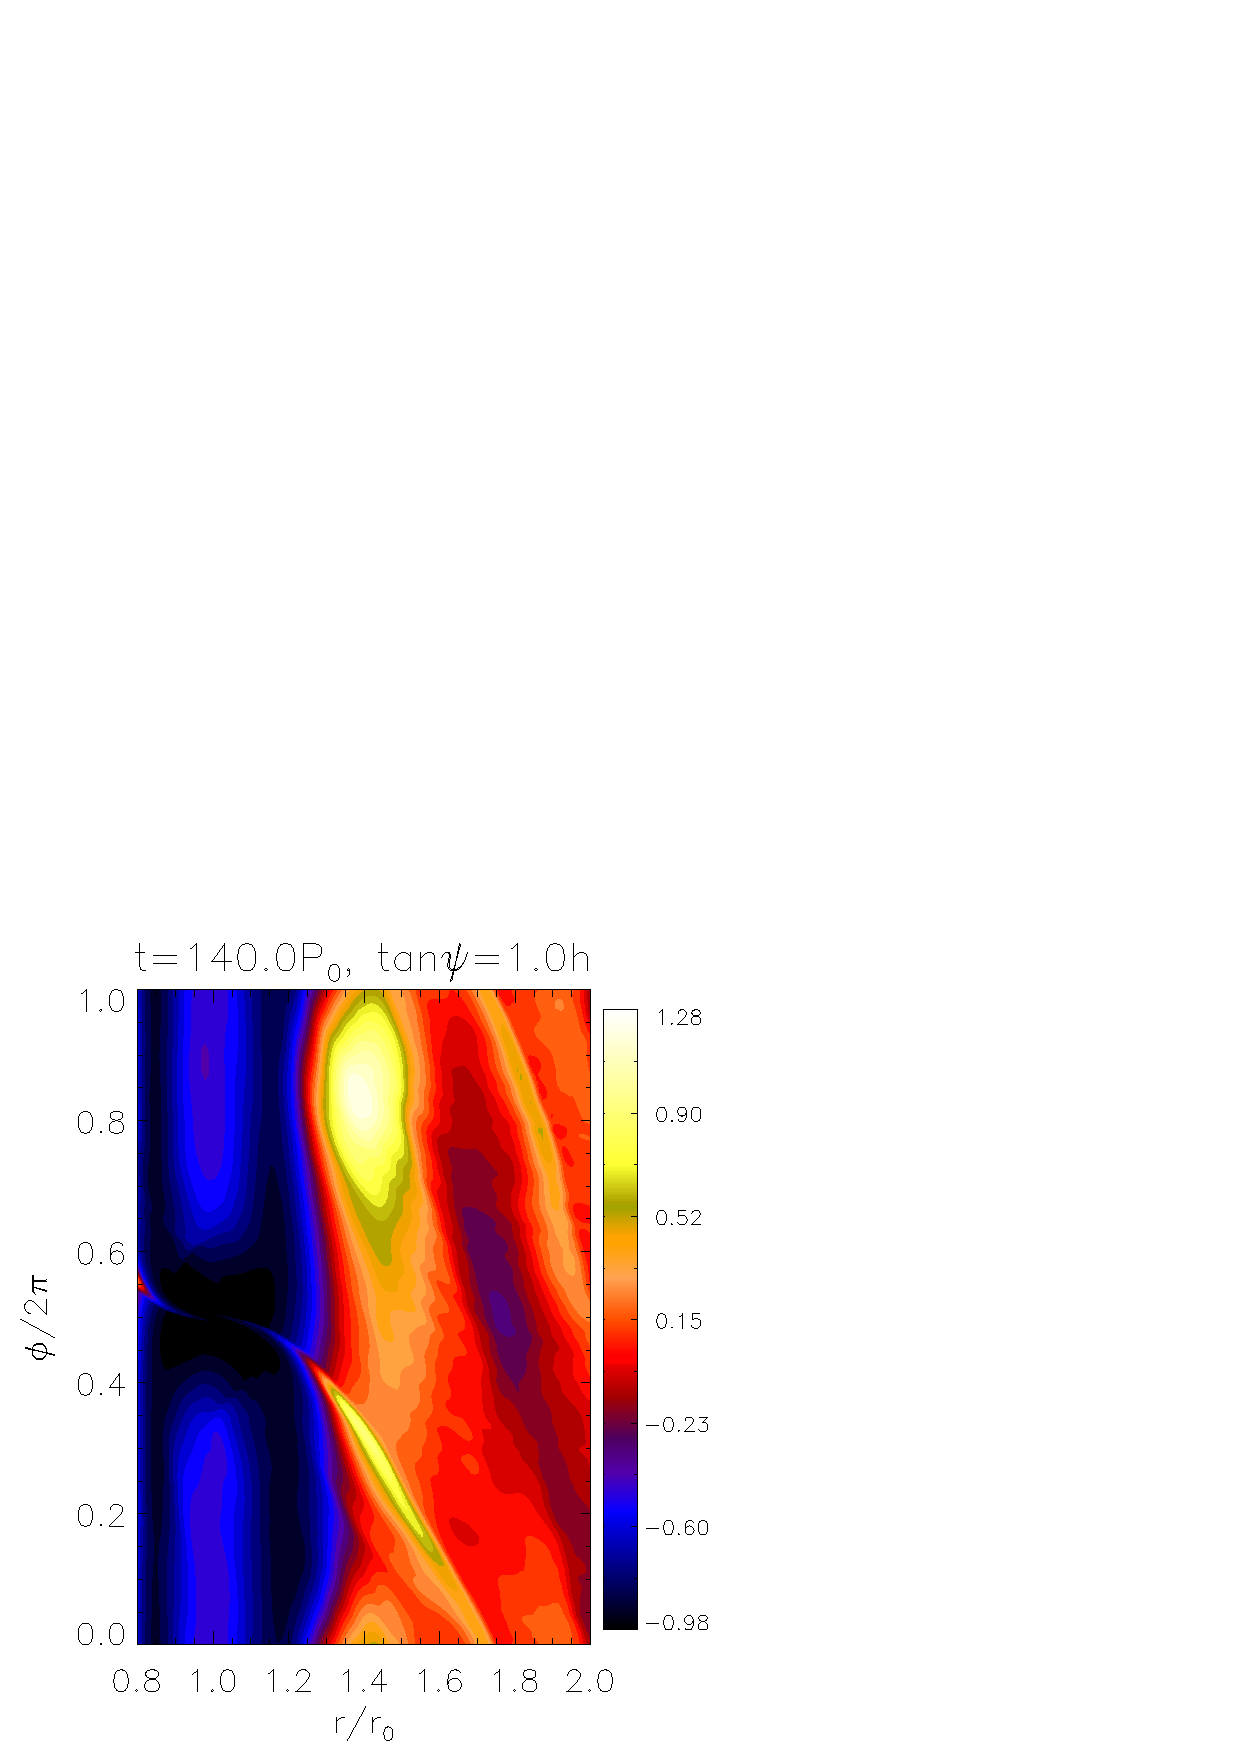
\includegraphics[scale=.27,clip=true,clip=true,trim=2.3cm 
     %% 1.84cm 0cm
     %% 0cm]{figures/jup0_pdisk014}\\
   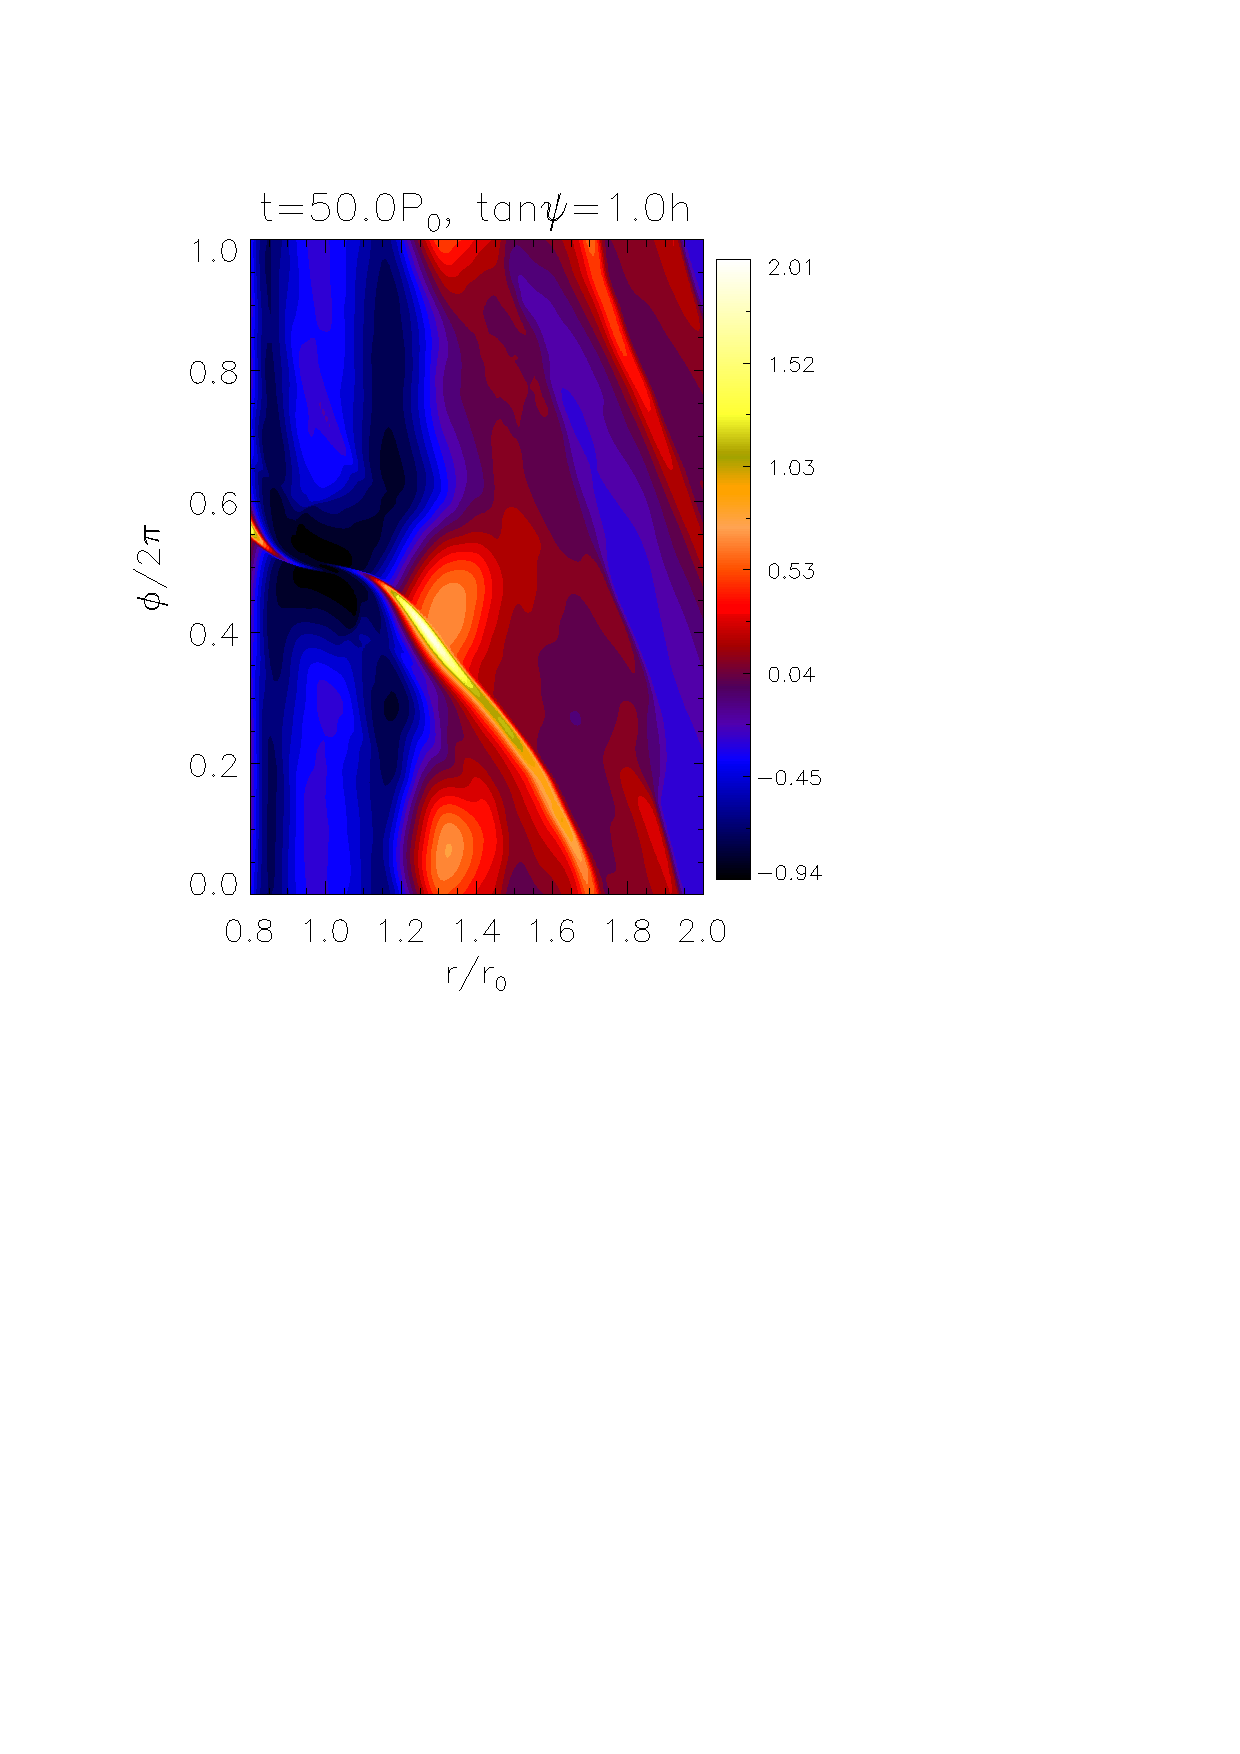
\includegraphics[scale=.39,clip=true,trim=0cm 1.84cm 0.0cm
     0.99cm]{figures/jup2_nuamp10_pdisk005}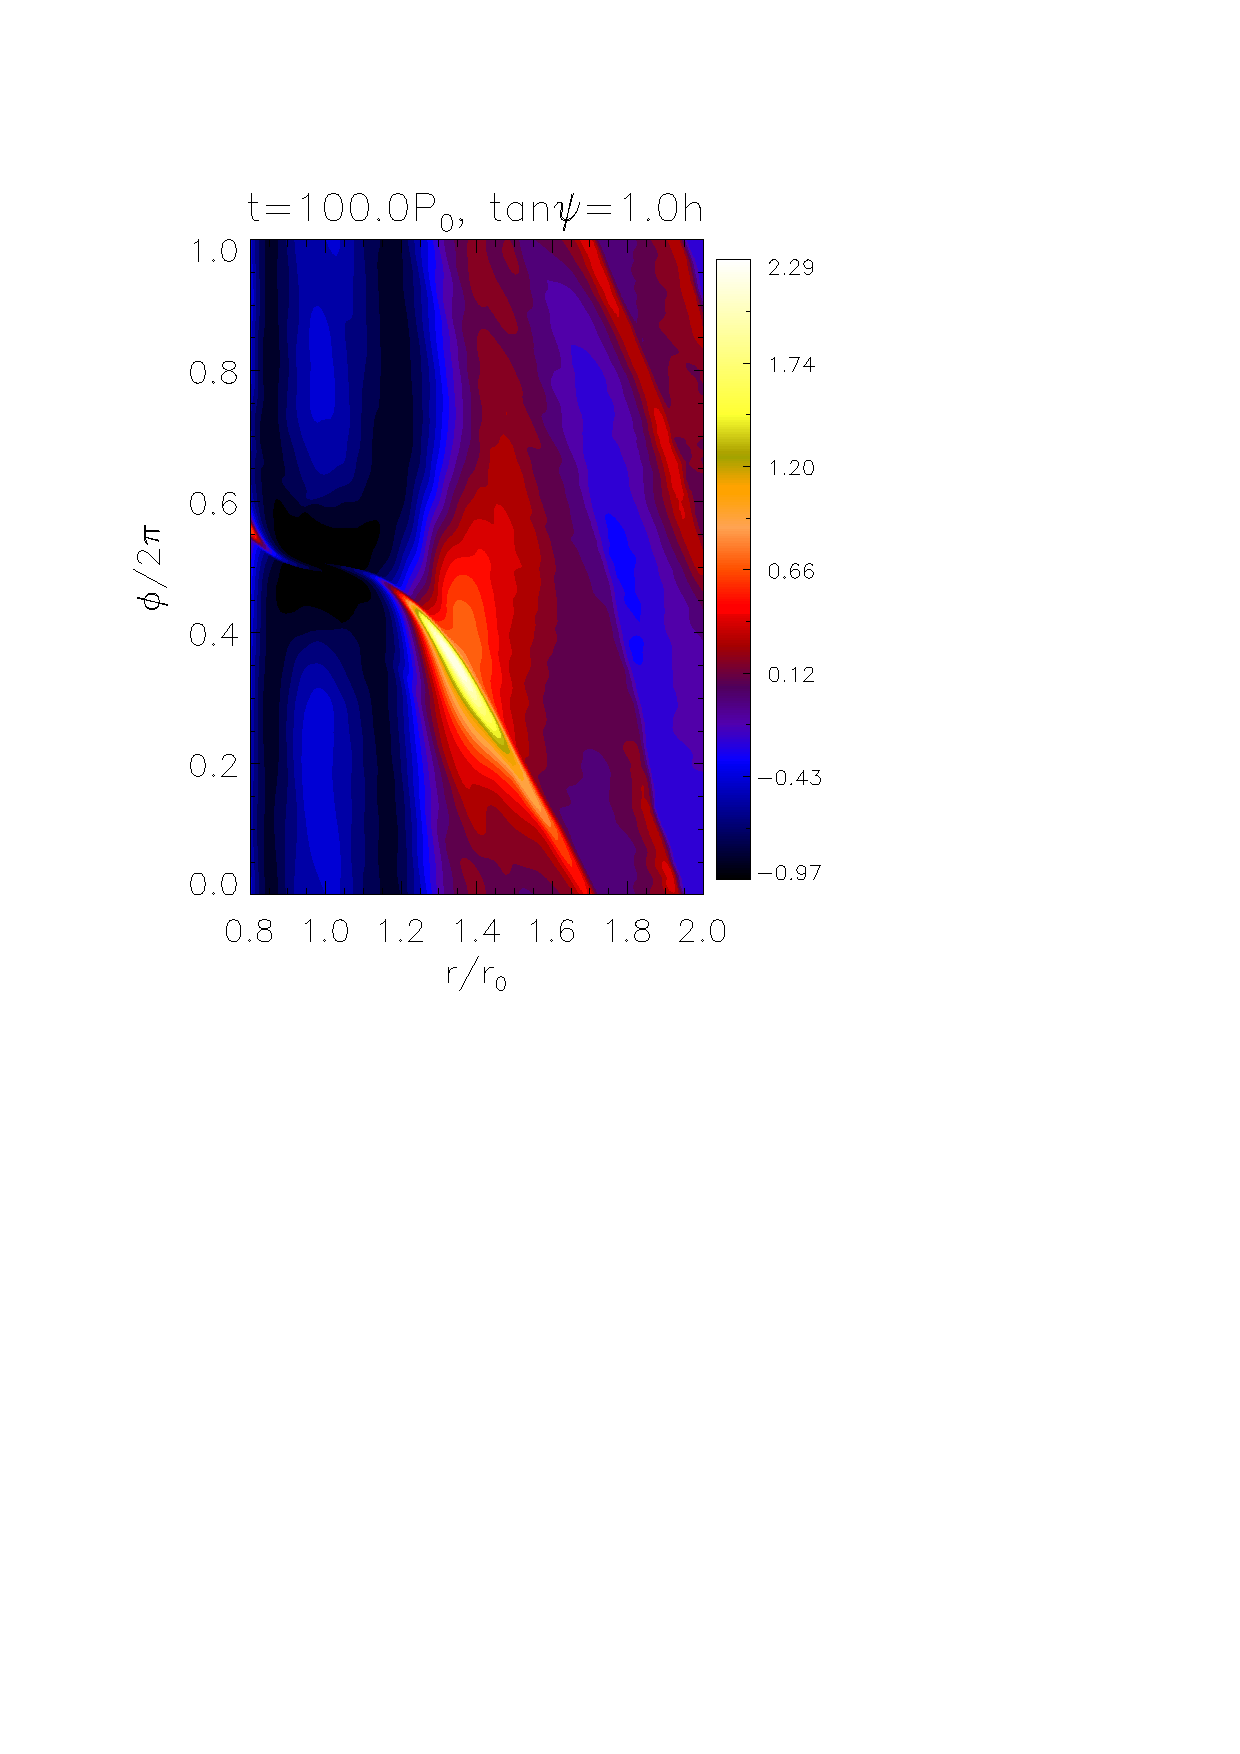
\includegraphics[scale=.39,clip=true,trim=2.3cm
     1.84cm 0.cm
     0.99cm]{figures/jup2_nuamp10_pdisk010}\\%% 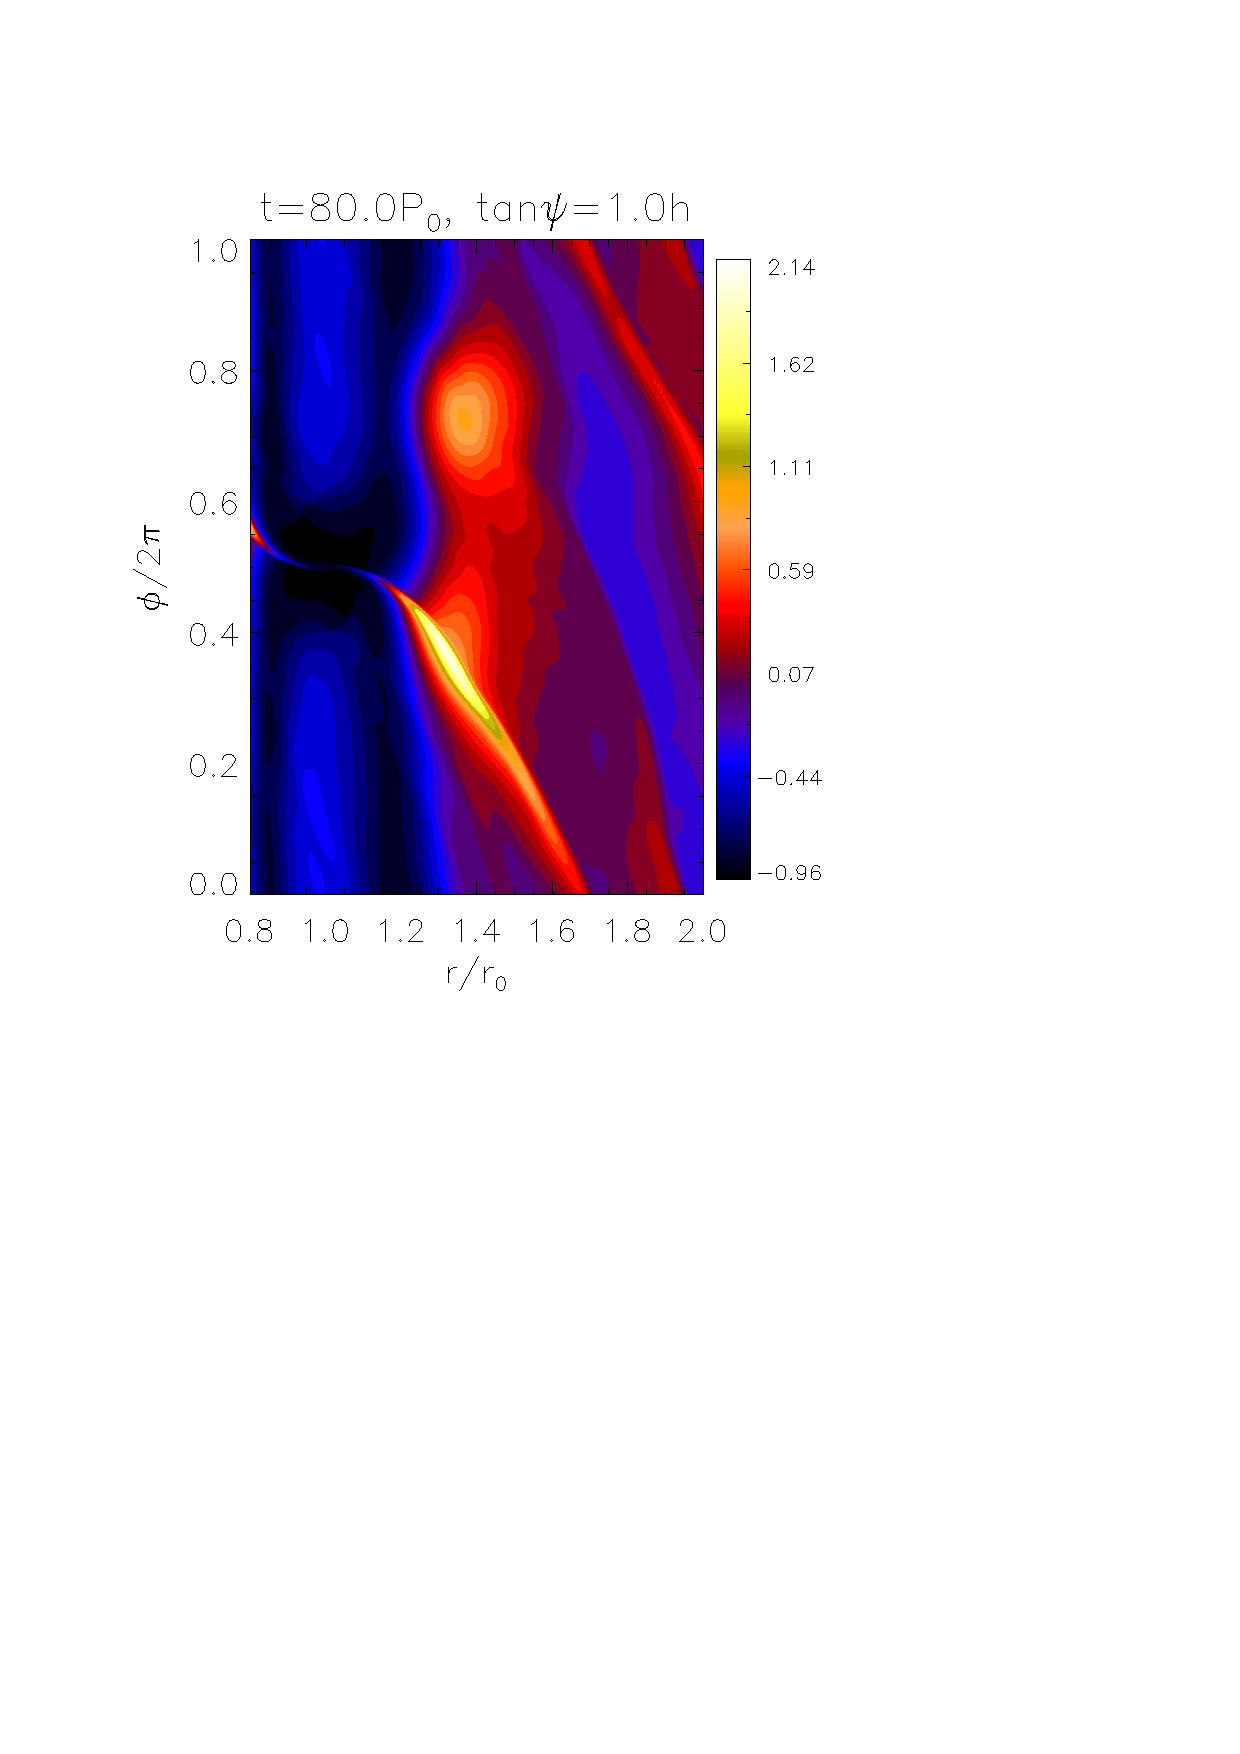
\includegraphics[scale=.27,clip=true,trim=2.3cm
     %% 1.84cm 0.cm
     %% 0.99cm]{figures/jup2_nuamp10_pdisk008}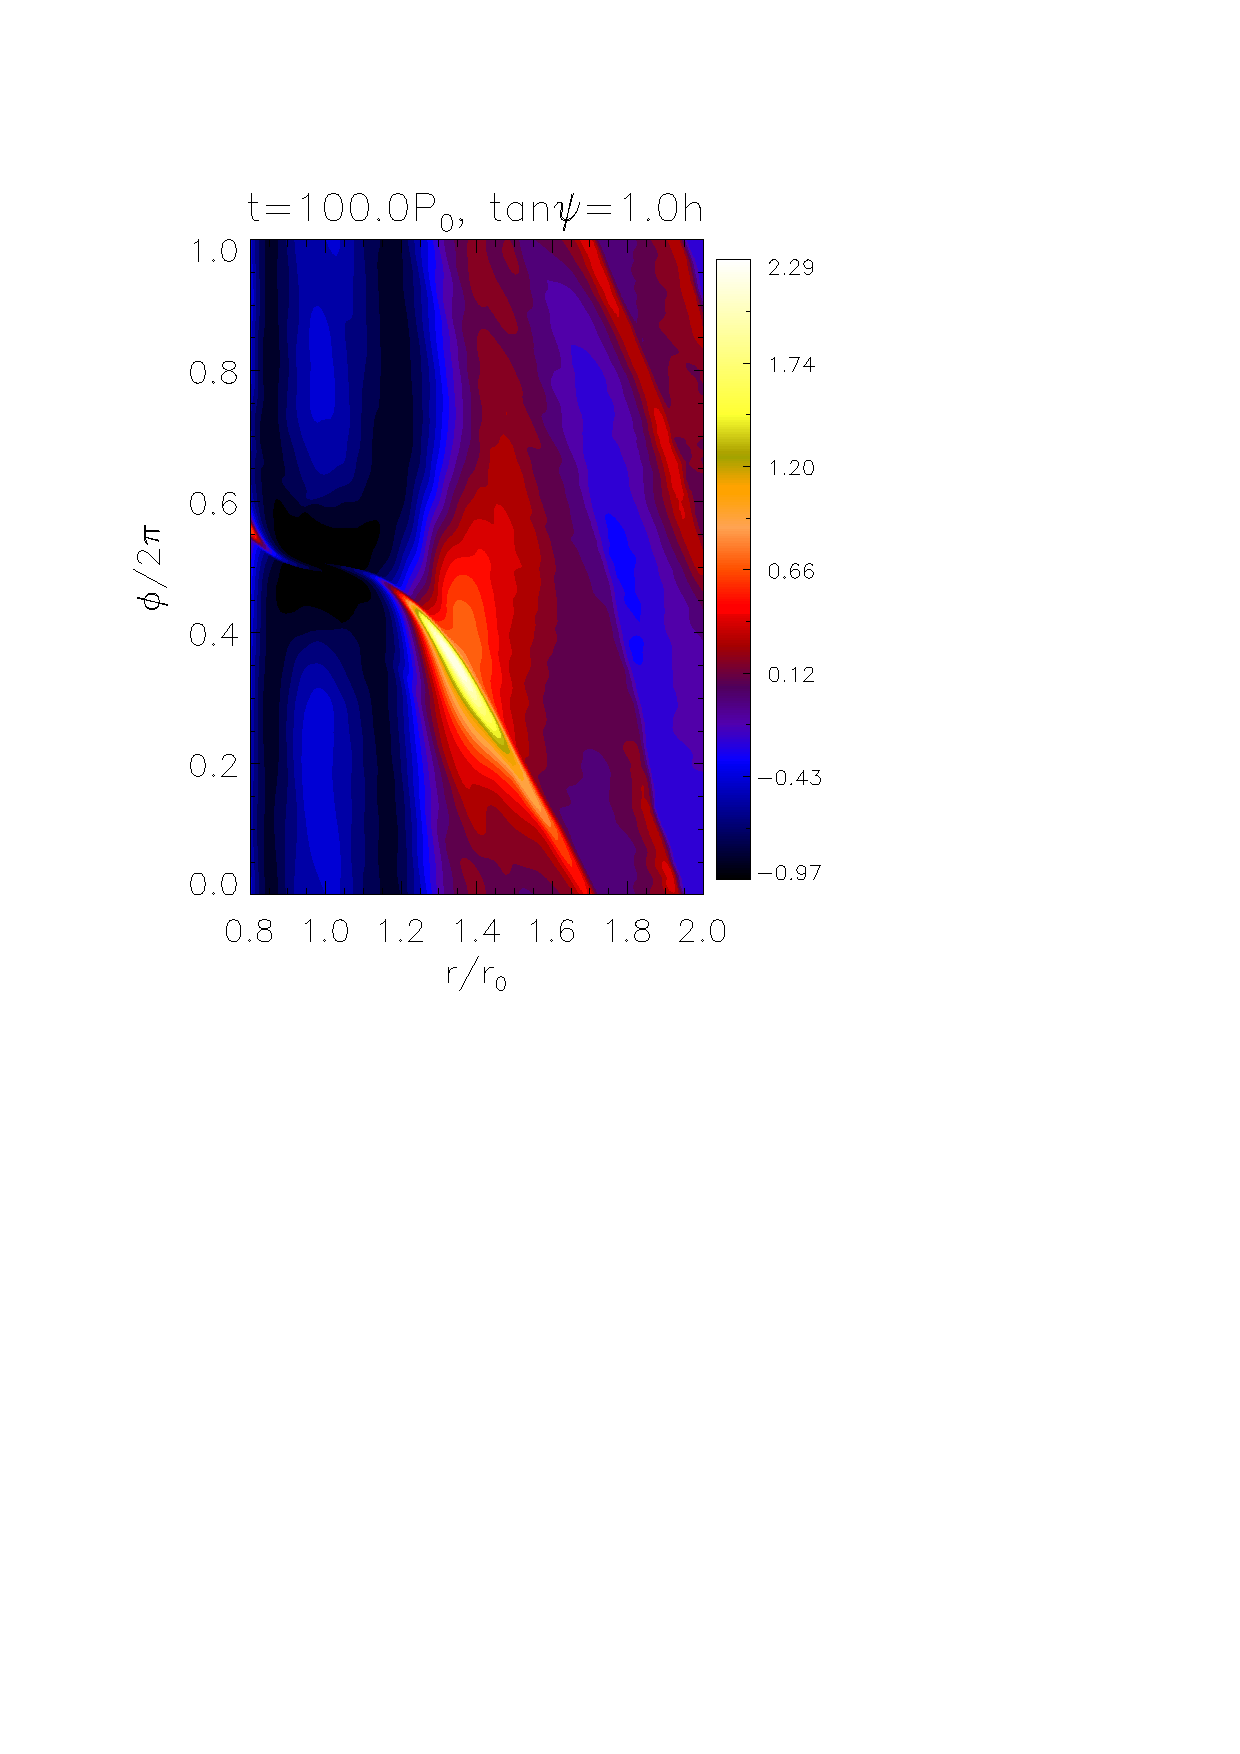
\includegraphics[scale=.27,clip=true,trim=2.3cm
     %% 1.84cm 0.cm
     %% 0.99cm]{figures/jup2_nuamp10_pdisk010}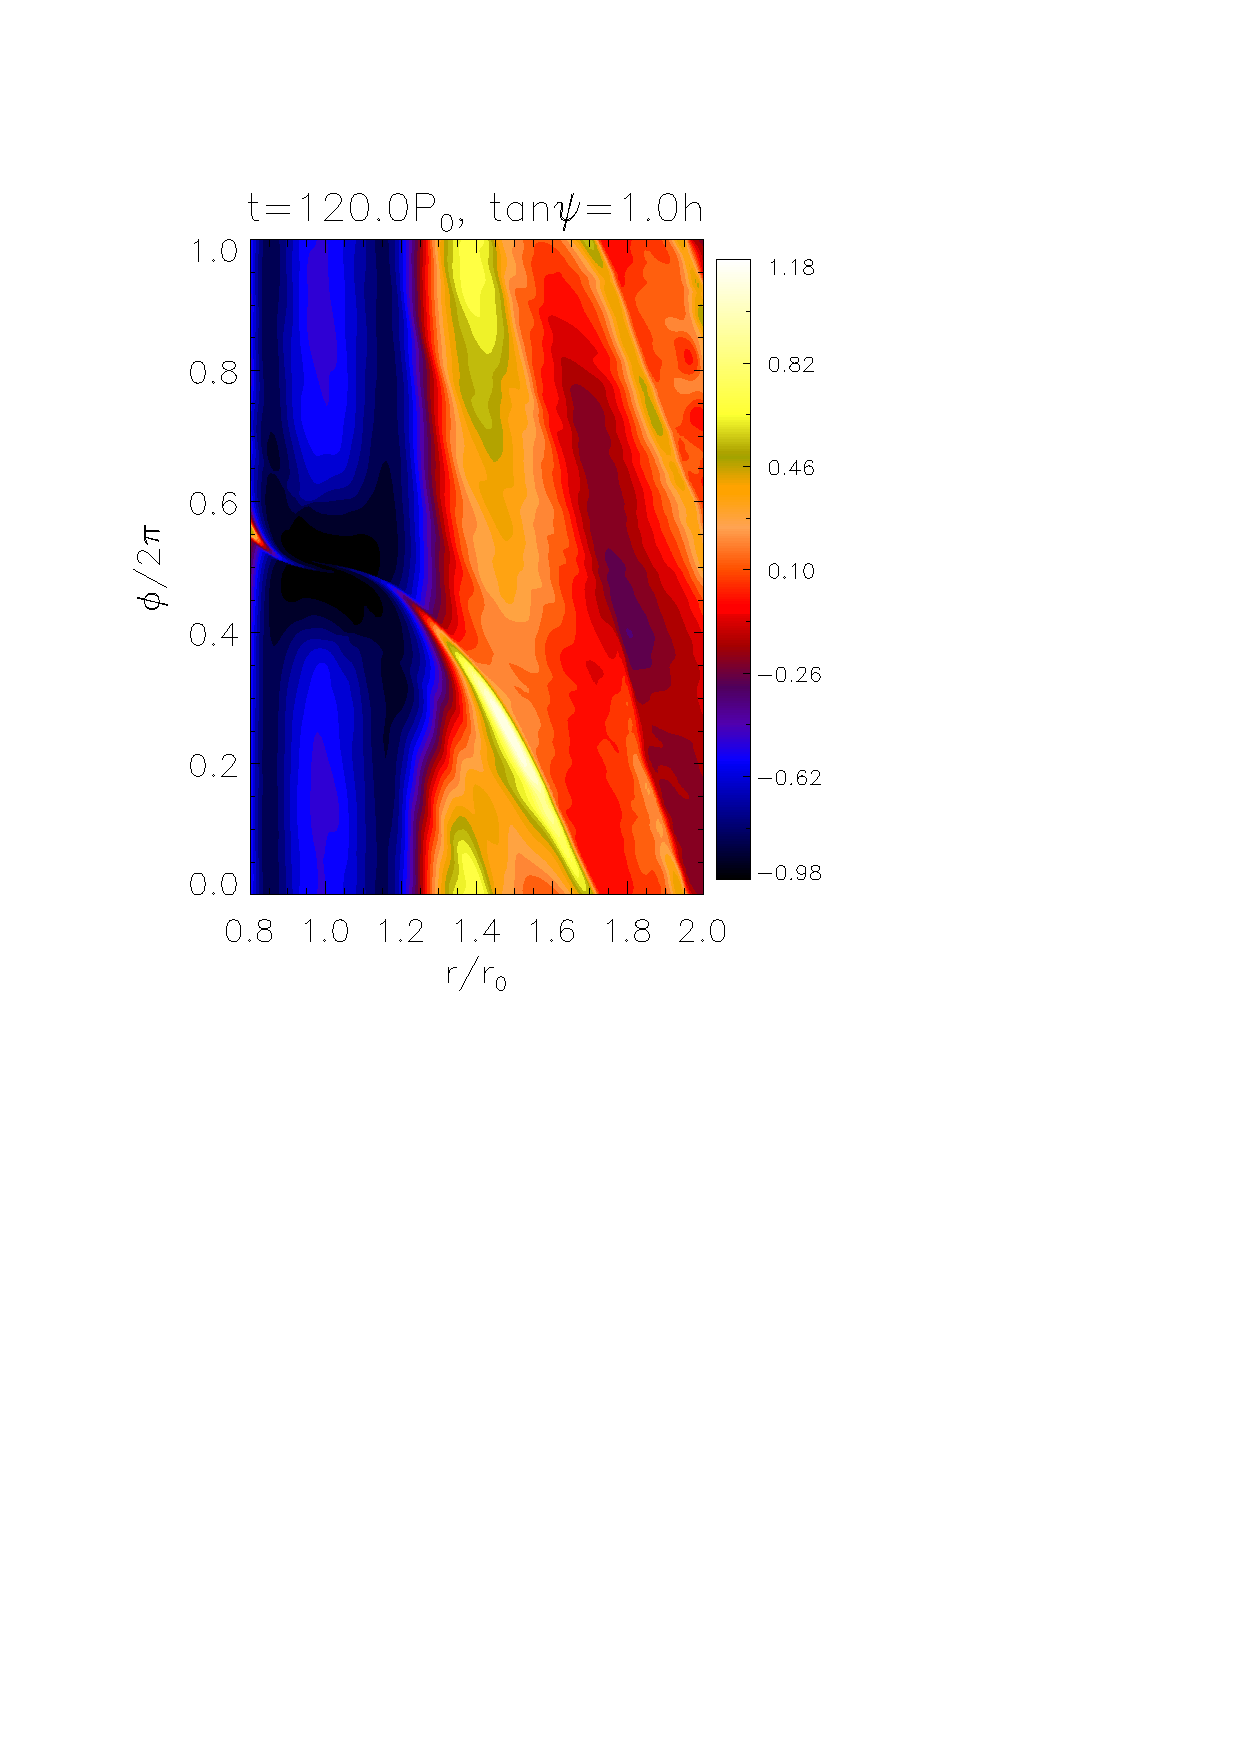
\includegraphics[scale=.27,clip=true,trim=2.3cm
     %% 1.84cm 0.cm
     %% 0.99cm]{figures/jup2_nuamp10_pdisk012}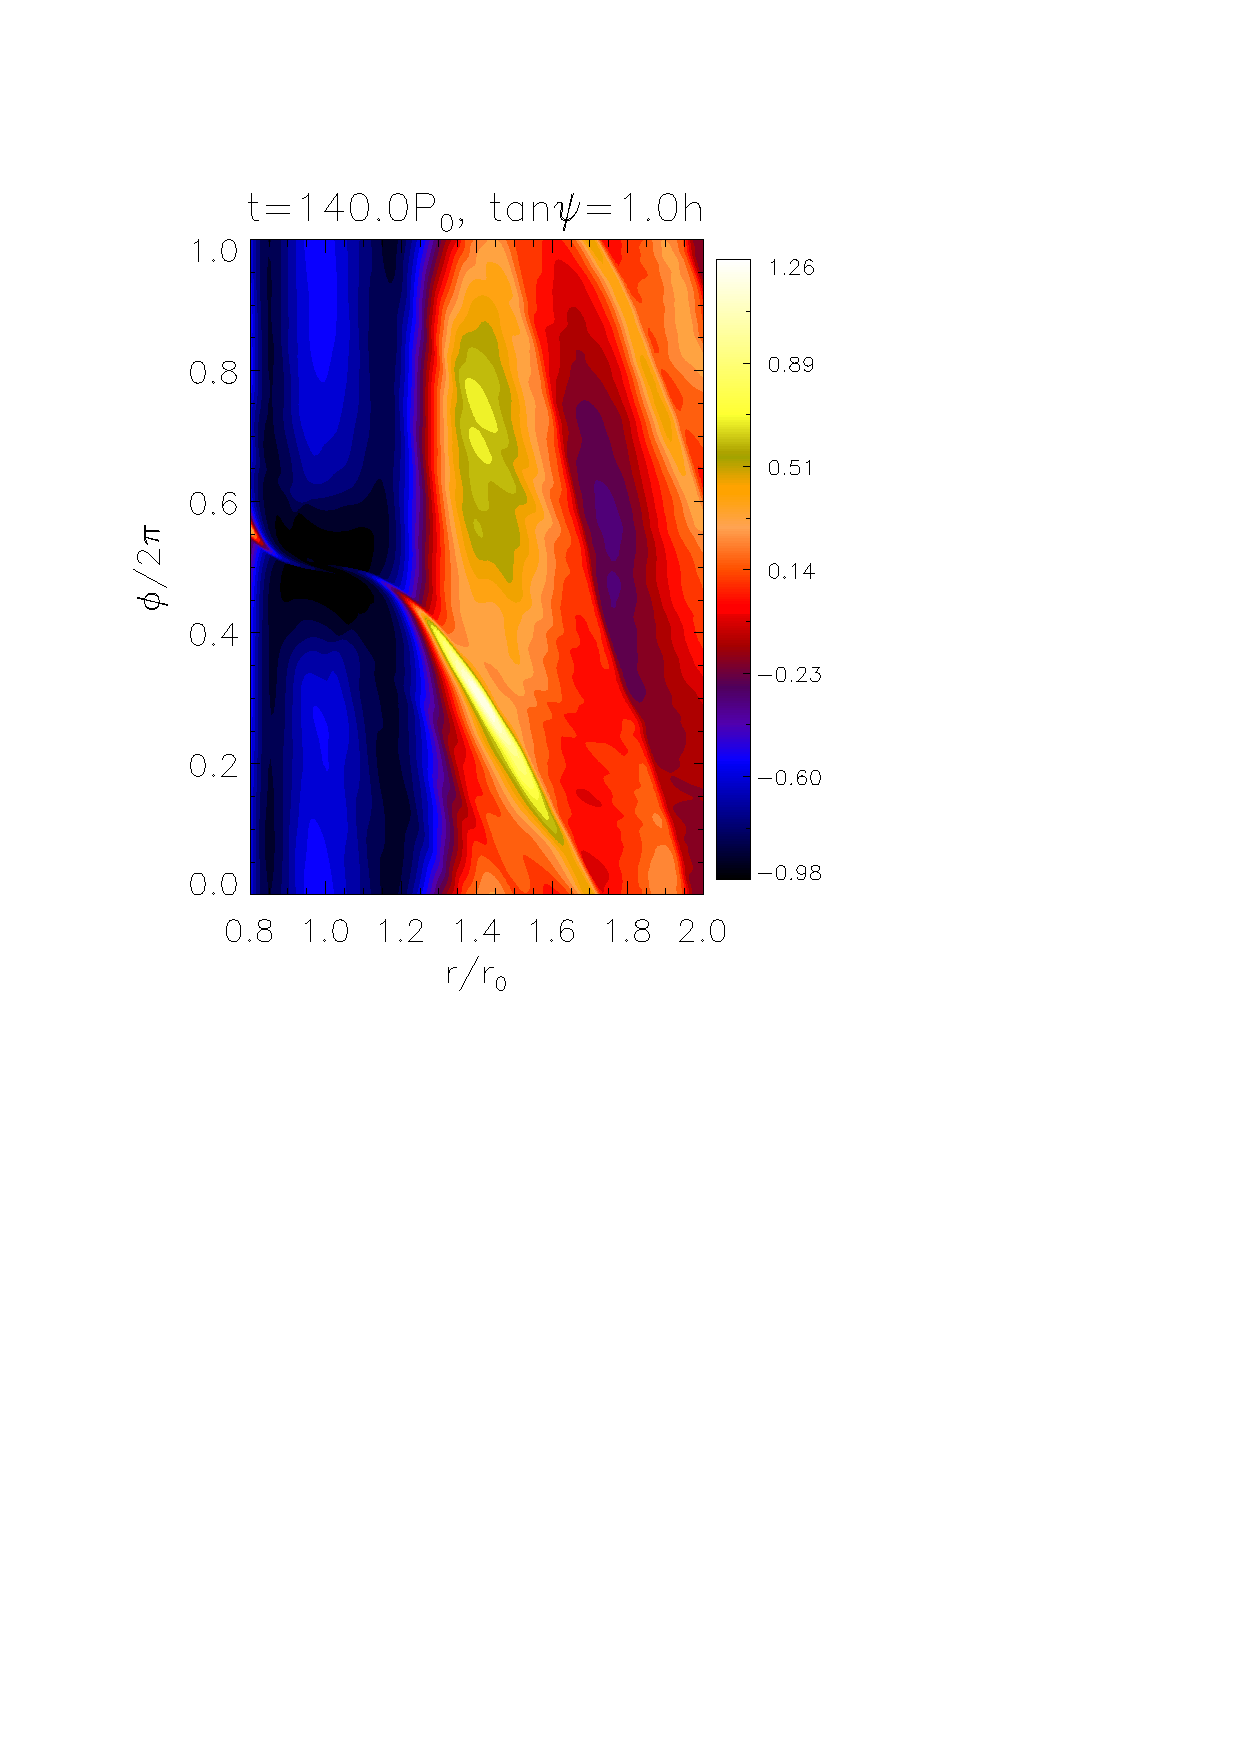
\includegraphics[scale=.27,clip=true,clip=true,trim=2.3cm
     %% 1.84cm 0.cm
     %% 0.99cm]{figures/jup2_nuamp10_pdisk014} \\
   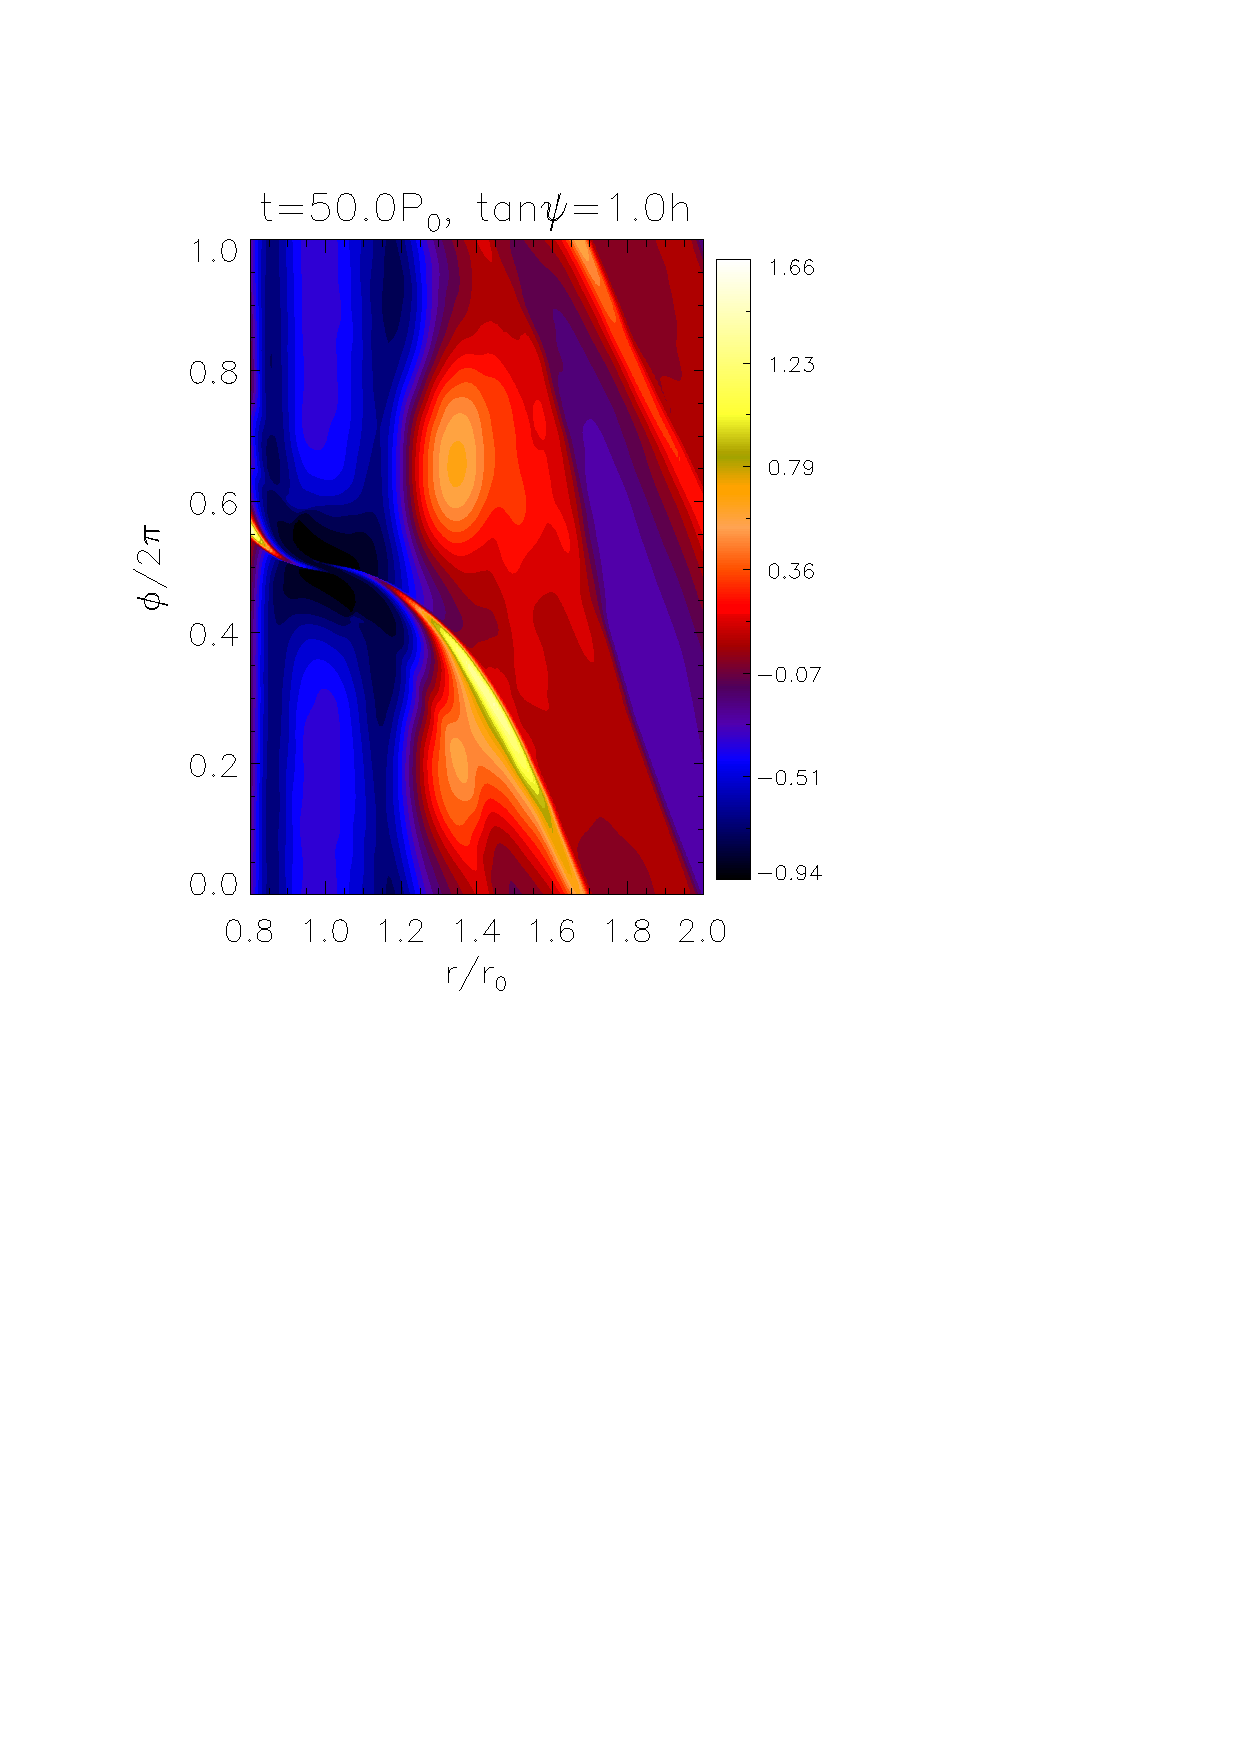
\includegraphics[scale=.39,clip=true,trim=0cm 0.cm 0.0cm
     0.99cm]{figures/jup3_nuamp10_pdisk005}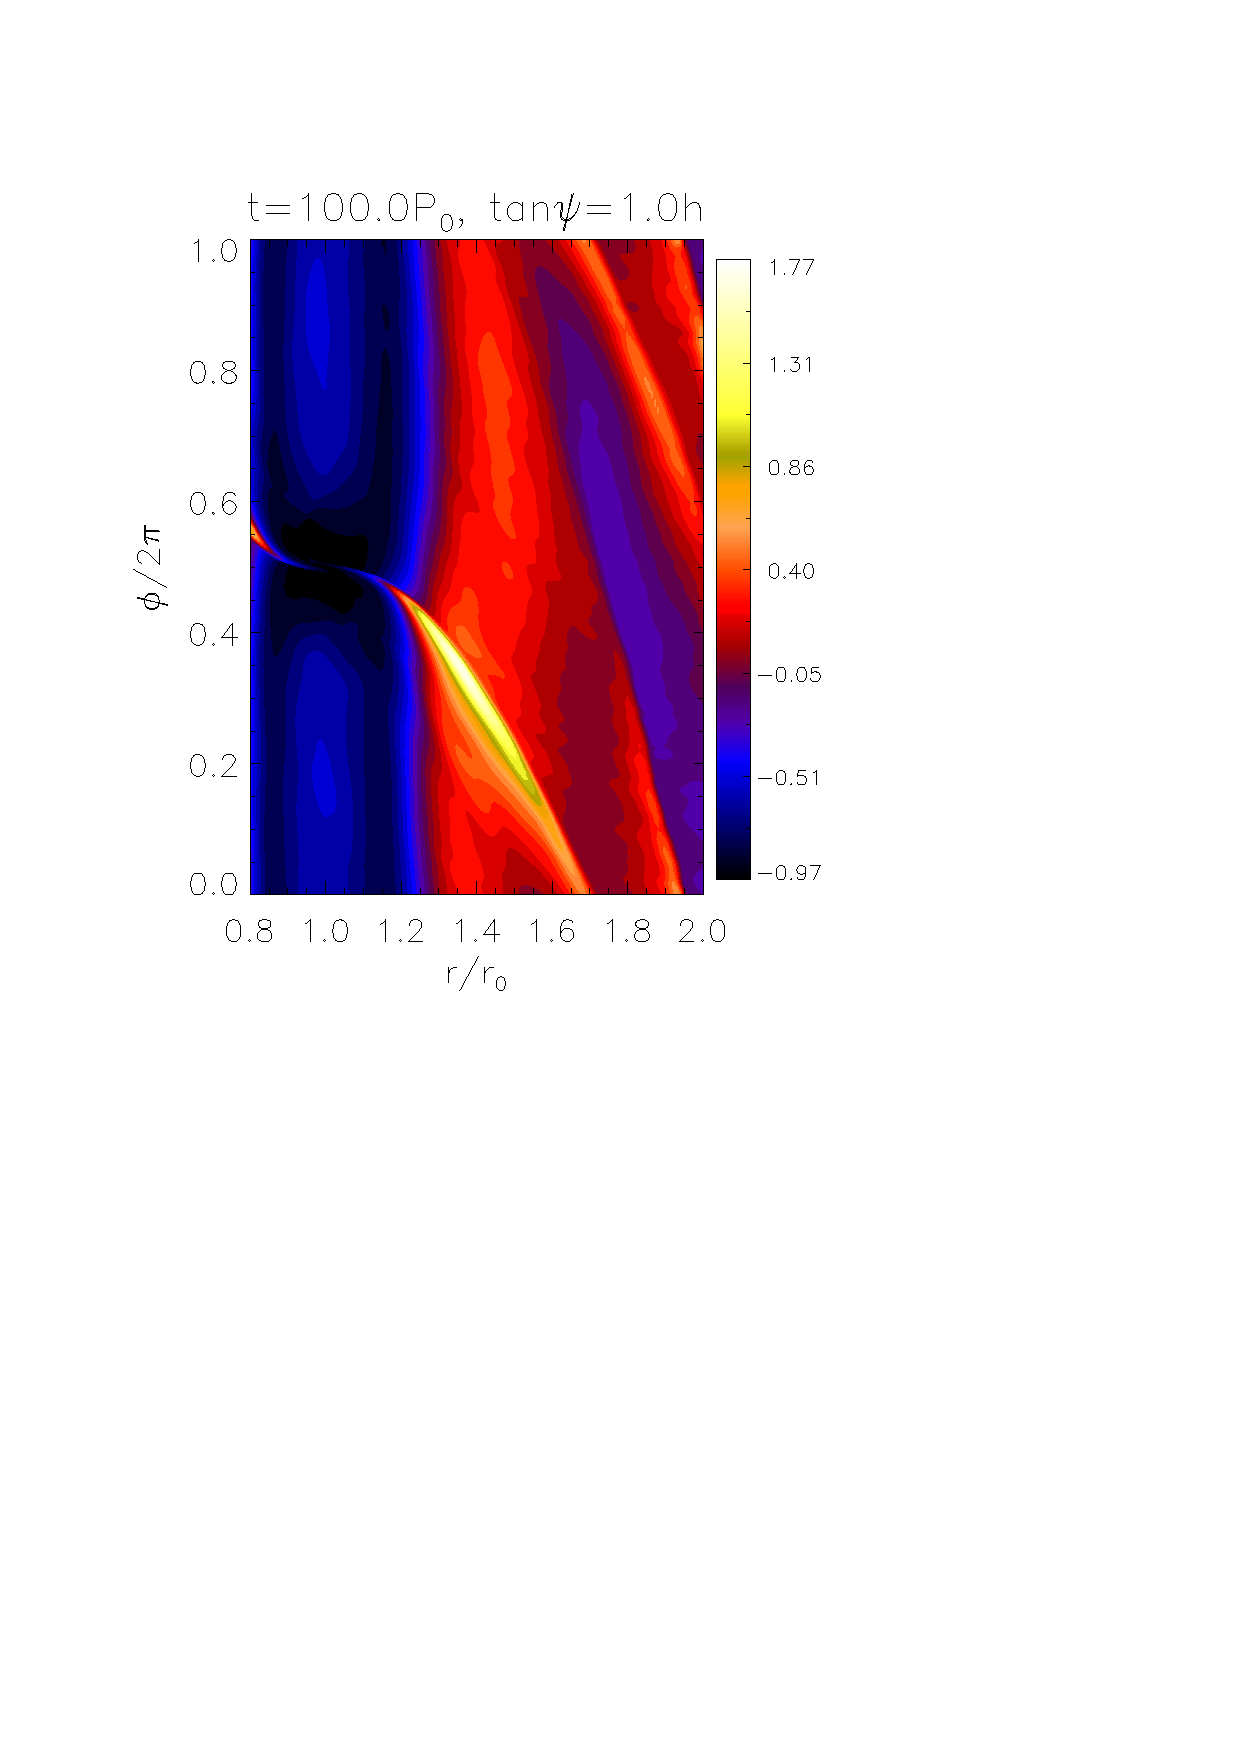
\includegraphics[scale=.39,clip=true,trim=2.3cm
     0.cm 0.cm
     0.99cm]{figures/jup3_nuamp10_pdisk010}\\%% 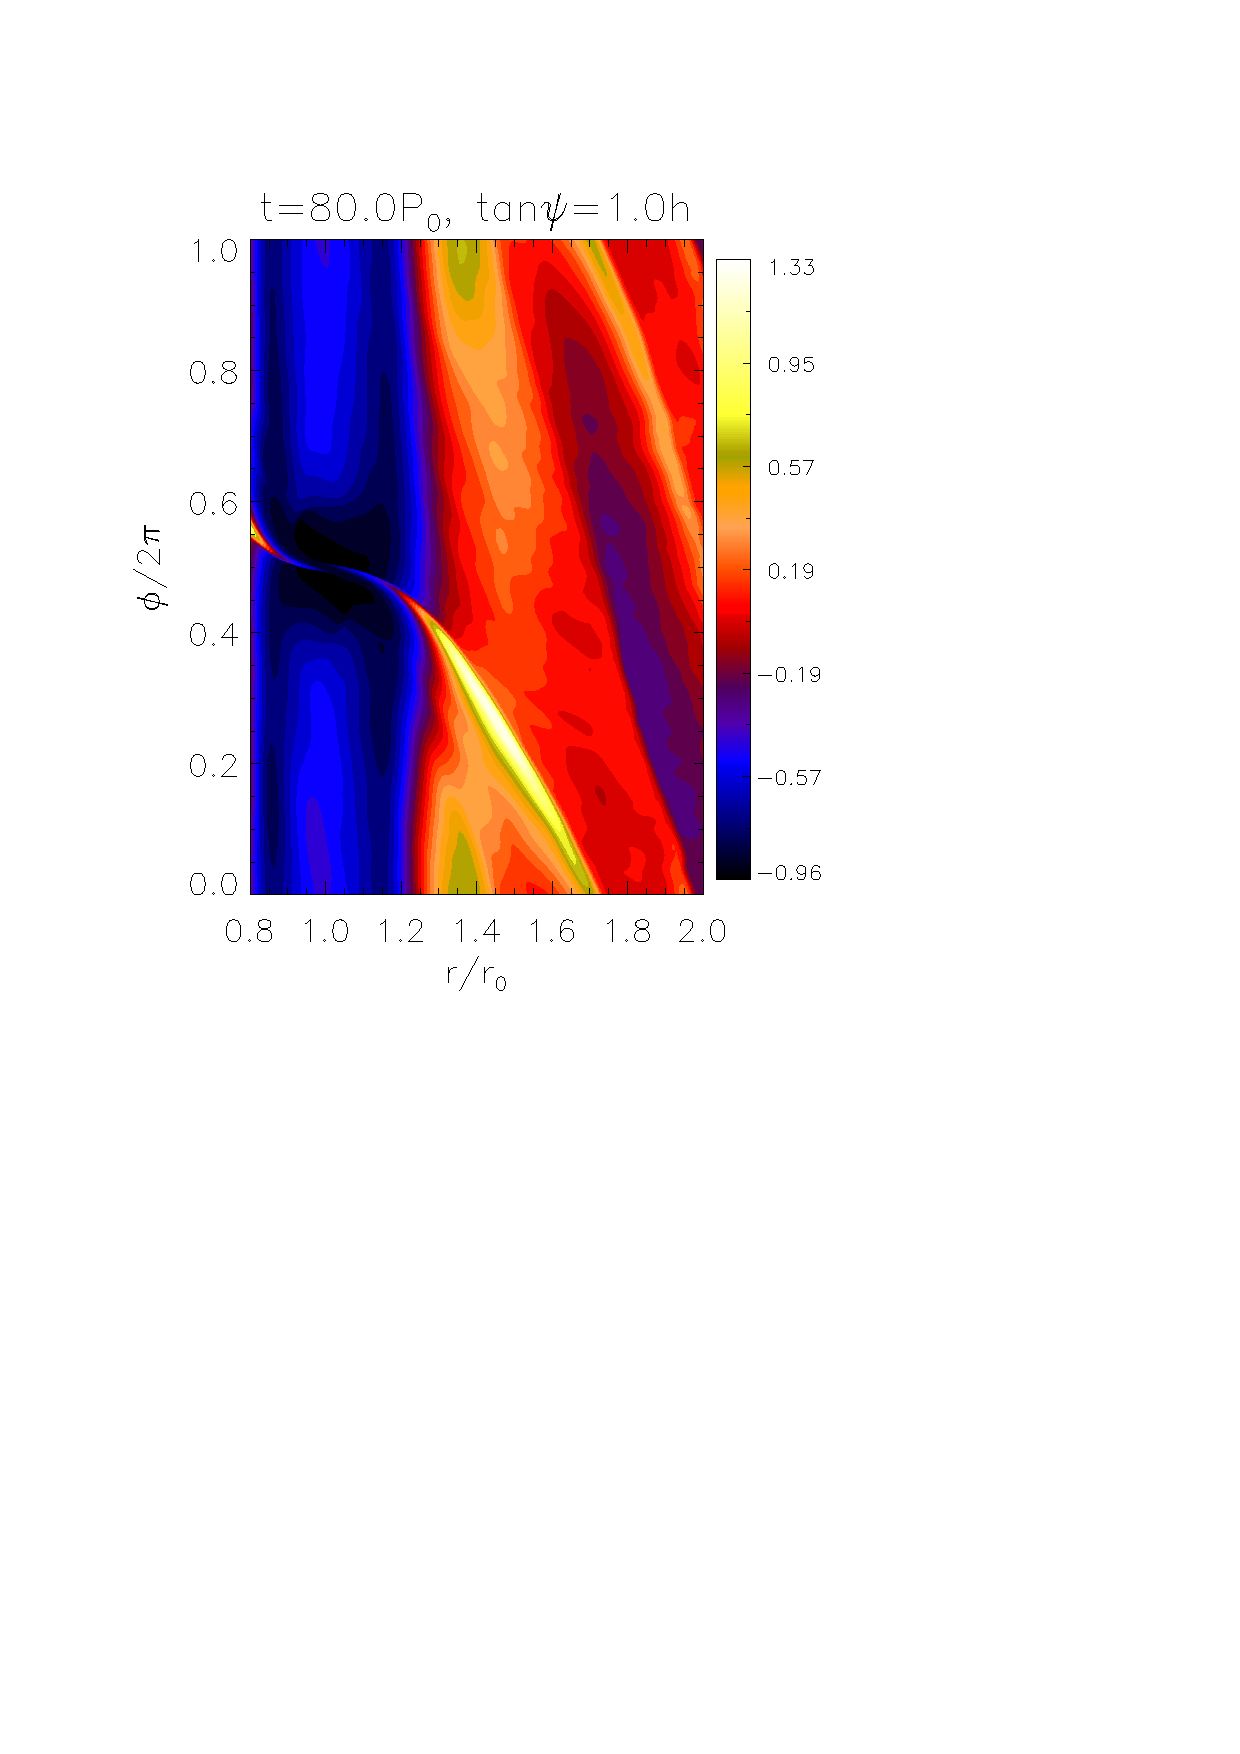
\includegraphics[scale=.27,clip=true,trim=2.3cm
     %% 0.cm 0.cm
     %% 0.99cm]{figures/jup3_nuamp10_pdisk008}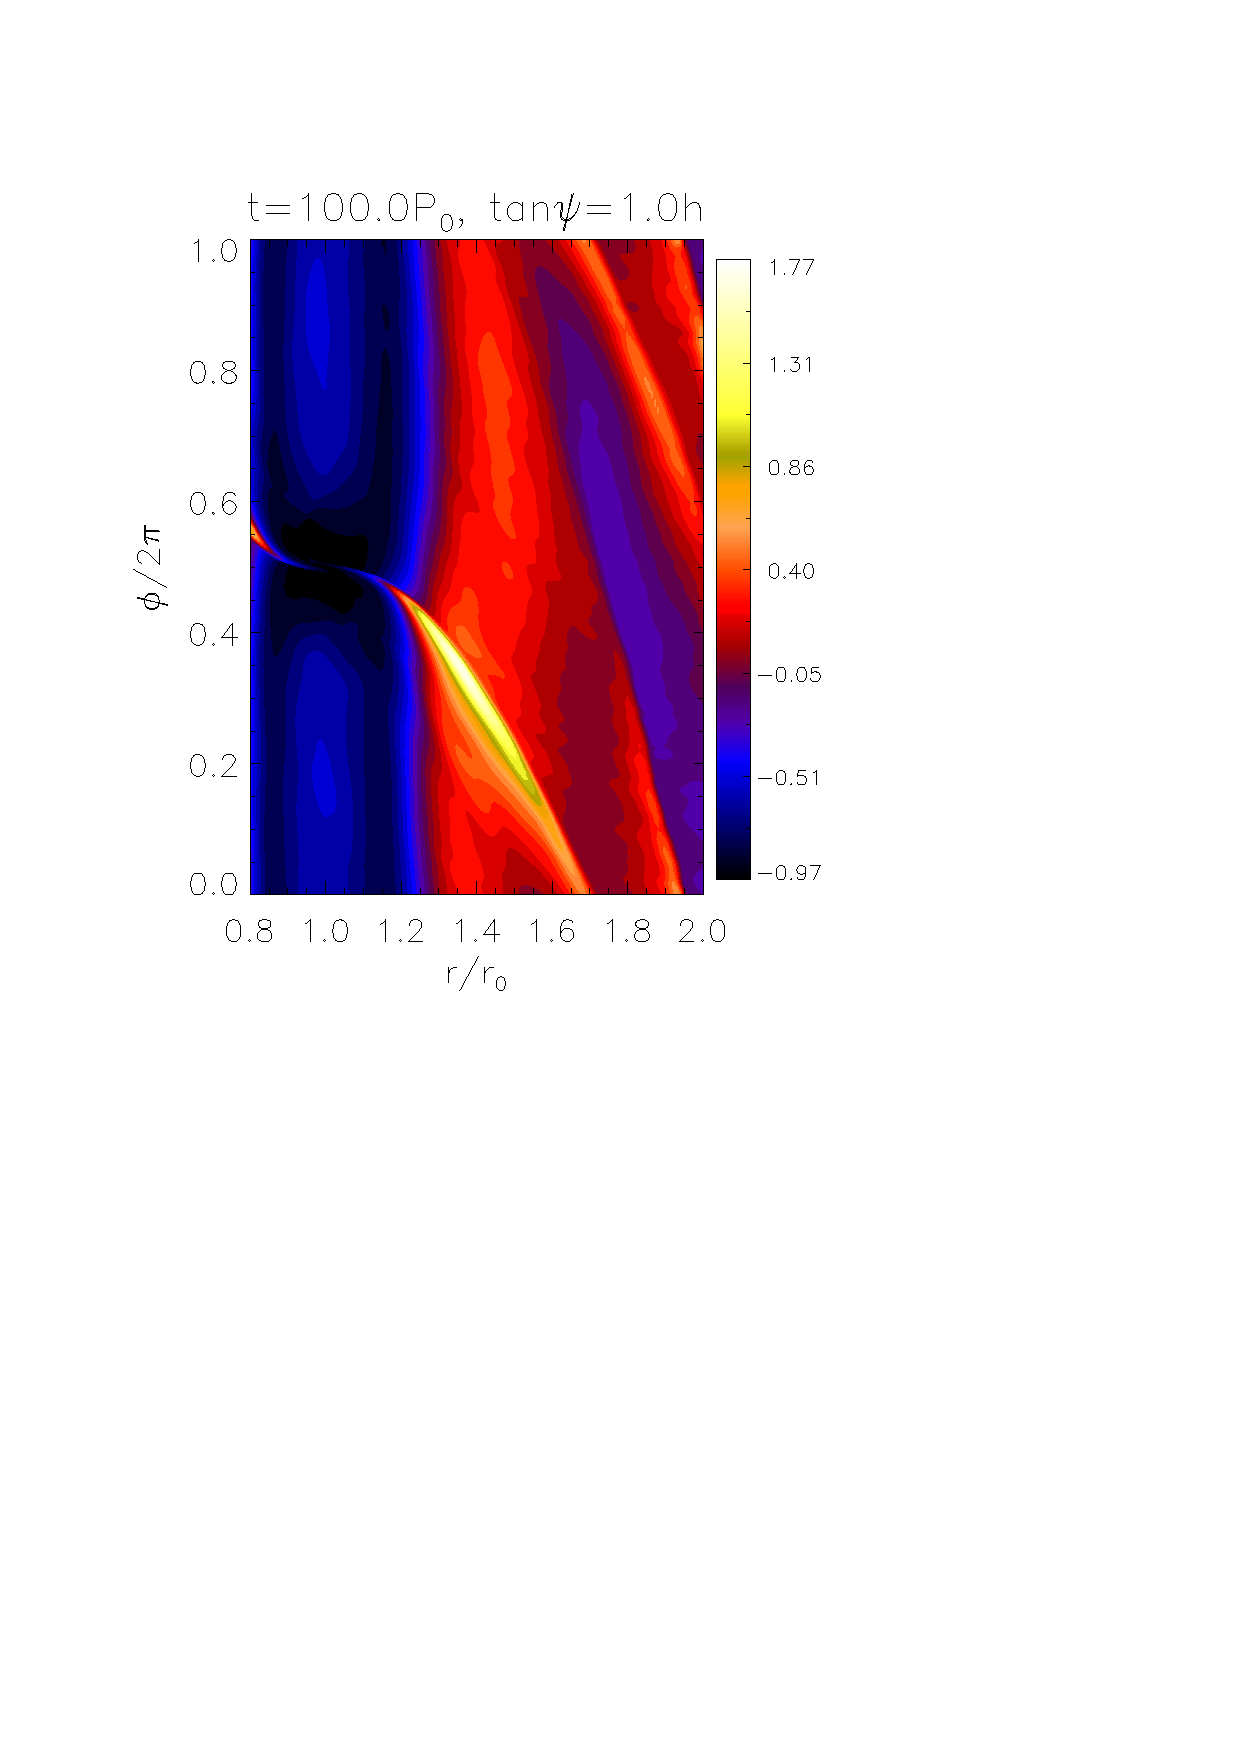
\includegraphics[scale=.27,clip=true,trim=2.3cm
     %% 0.cm 0.cm
     %% 0.99cm]{figures/jup3_nuamp10_pdisk010}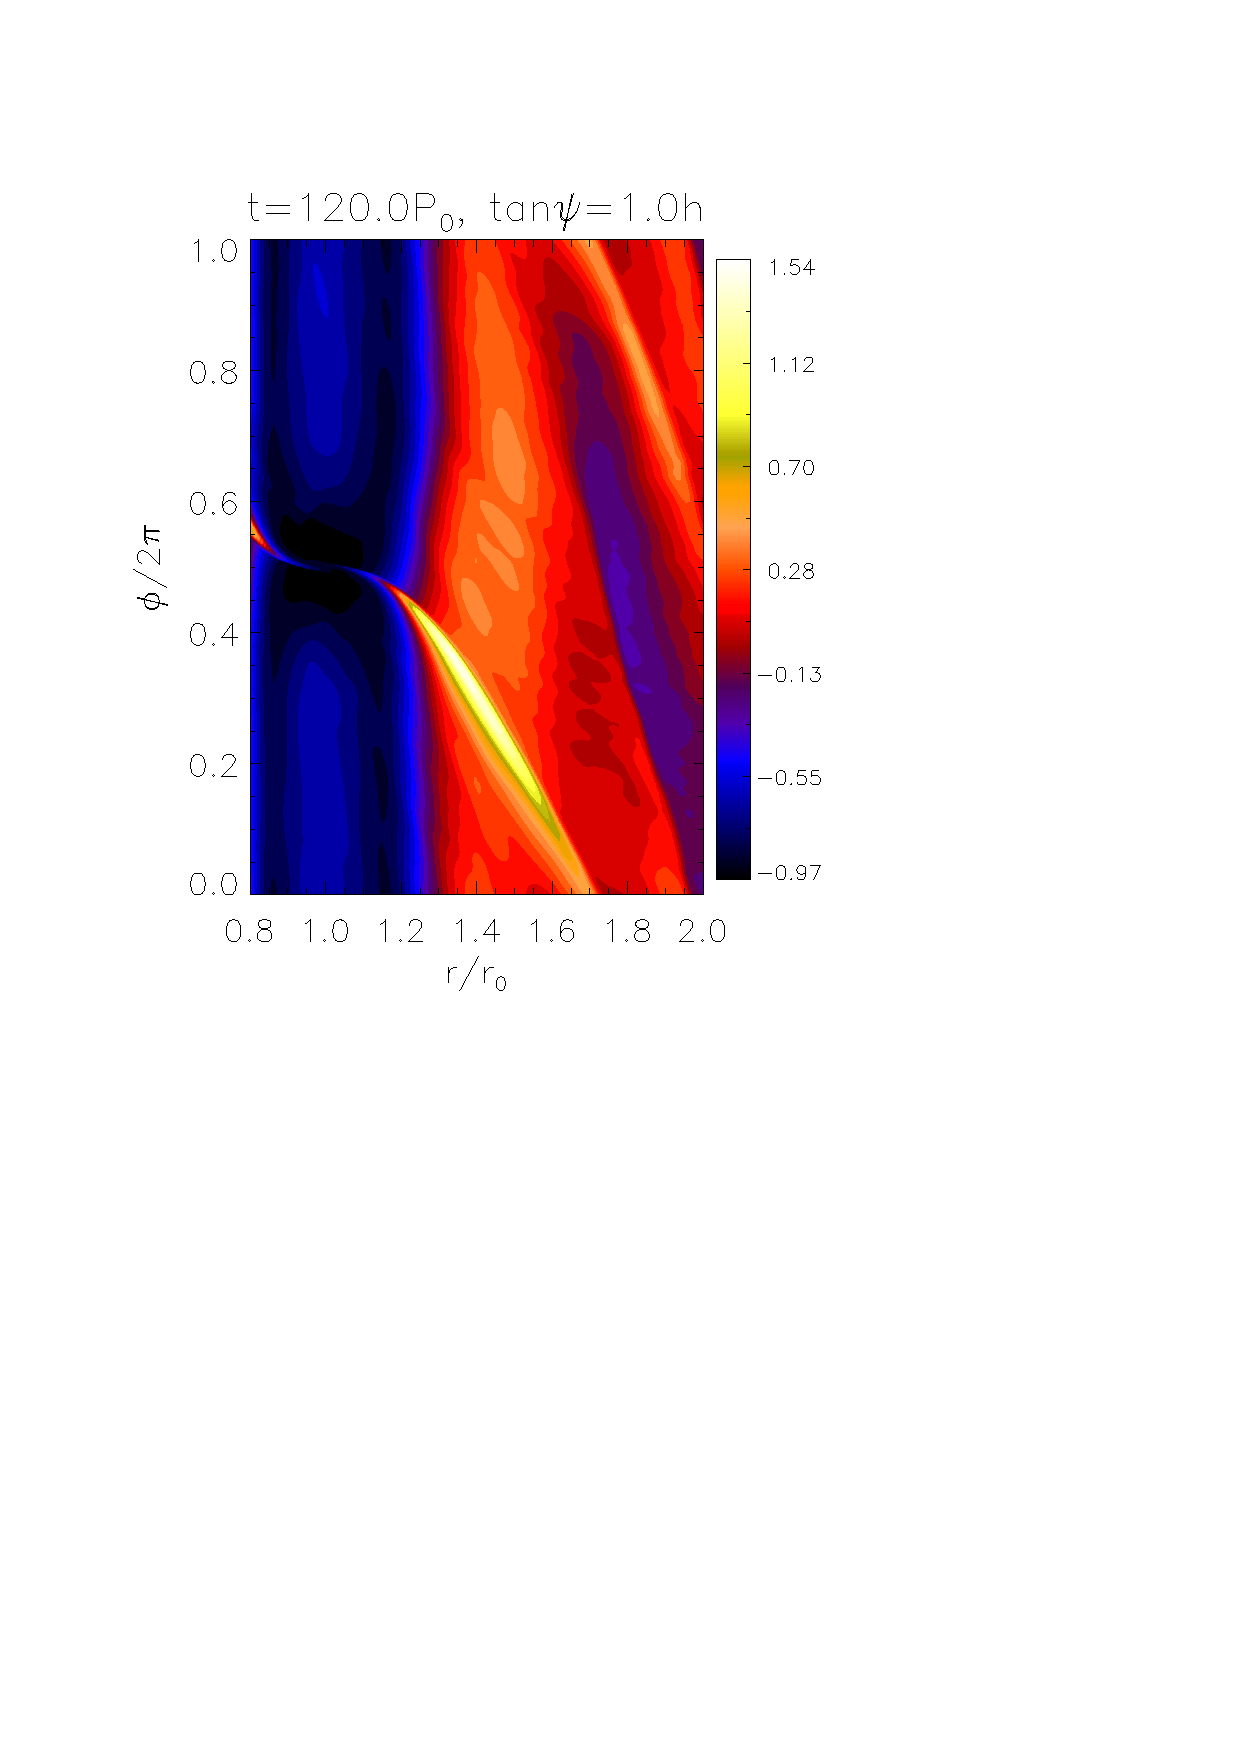
\includegraphics[scale=.27,clip=true,trim=2.3cm
     %% 0.cm 0.cm
     %% 0.99cm]{figures/jup3_nuamp10_pdisk012}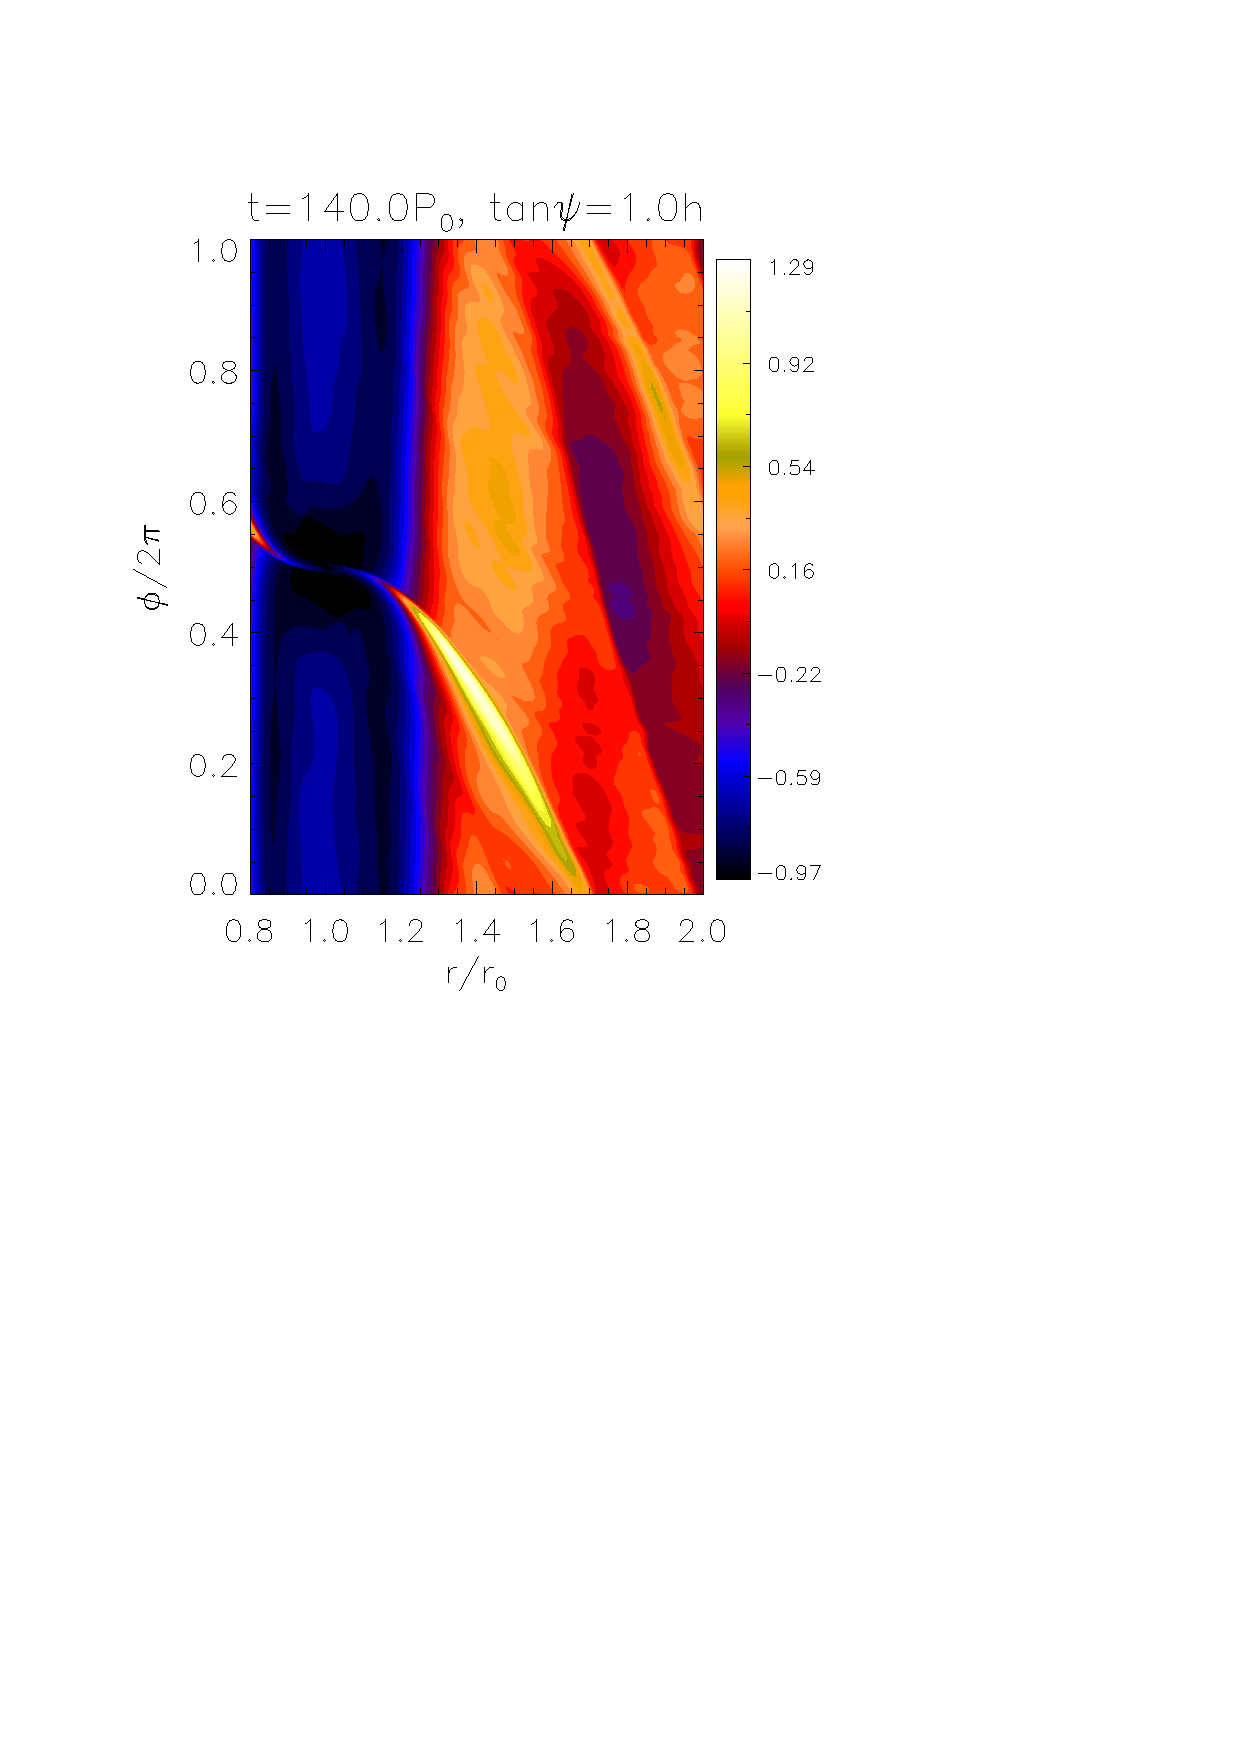
\includegraphics[scale=.27,clip=true,clip=true,trim=2.3cm
     %% 0.cm 0.cm
     %% 0.99cm]{figures/jup3_nuamp10_pdisk014} \\
   \caption{Density perturbation $\delta\rho$ for disc-planet
     simulations case P0 (top), P1 (middle) and P2 (bottom). The
     thickness of the viscous layer occupies $0\%,\,25\%$ and $50\%$
     of the uppermost vertical domain from top to bottom. 
   \label{jup0}}
 \end{figure}


\subsubsection{PV evolution}





\subsection{Viscous atmosphere}
%We now consider appending a viscous layer on top of the fiducial 
%case P0. 
Case P3 is the same as case P0 above, except with an increased
vertical domain size of $3H$. Case P4 has a high-viscosity layer with
$\hat{\nu}\sim10^{-4}$ in the the uppermost scale-height of the
computational domain. In other words, the bulk of the 
%% has a viscosity $\hat{\nu} \sim 10^{-5}$ and $\hat{\nu}\sim 10^{-4}$
%% for cases P3 and P4, respectively. 
disk for case P4 has a low-viscosity of $\hat{\nu}\sim10^{-6}$, but
with a viscous atmosphere appended on top.  

Fig. \ref{jup0_3h} shows the density pertubation at $t=100P_0$ for
cases P3 and P4. Case P3 is essentially identical to case P0, so the
vortex instability is not affected by vertical domain size. We note
that the viscosity is increased in the disc atmosphere, where the
density is a factor $\sim 7$ times smaller than the midplane (but the
viscosity is $100$ times larger). The viscous layer has surpressed
vortex formation via the RWI. This implies that vortex formation via
the RWI at planetary gap edges can not tolerate a signigicantly
viscous atmosphere, even if such a layer only occurs away from the
midplane.    

\begin{figure}
   \centering
   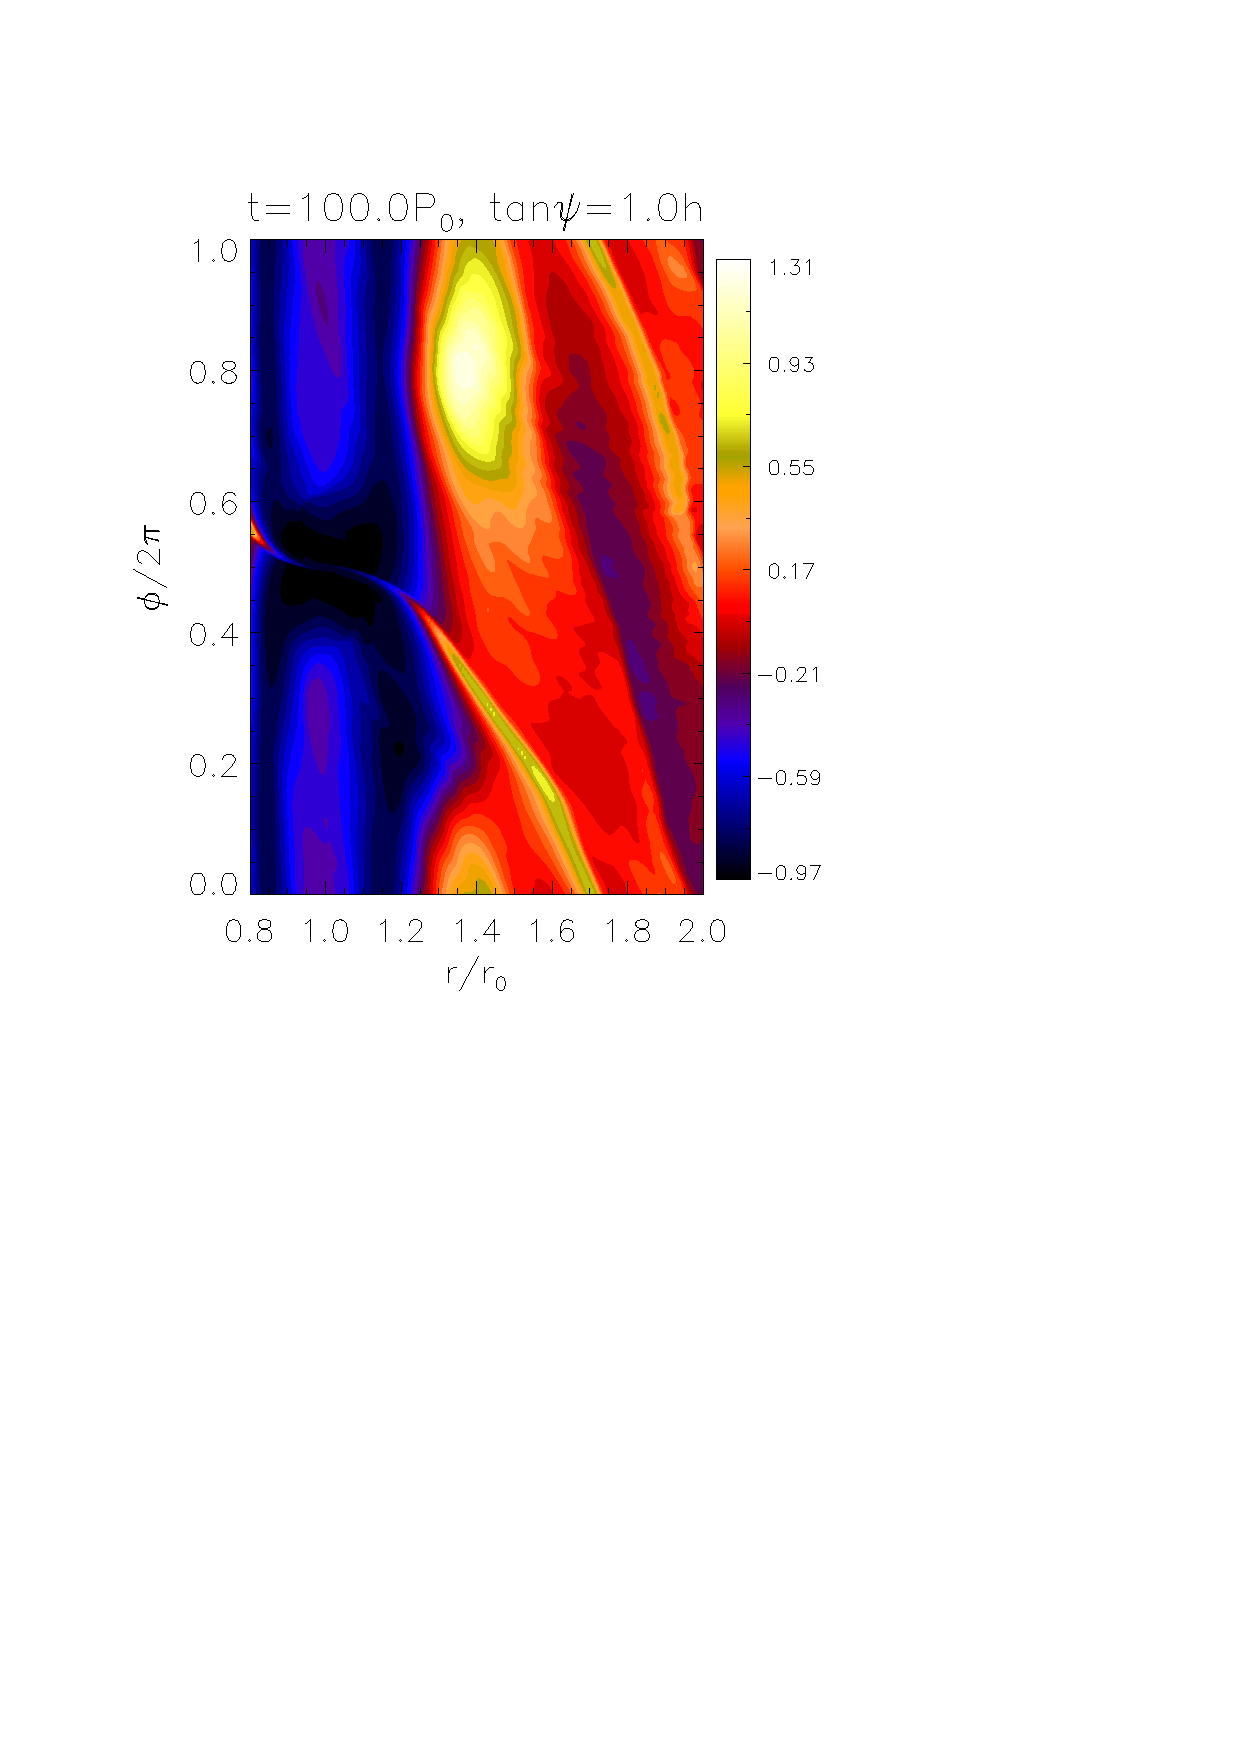
\includegraphics[scale=.39,clip=true,trim=0cm 1.84cm 0cm
     0cm]{figures/jup0_3h_pdisk010}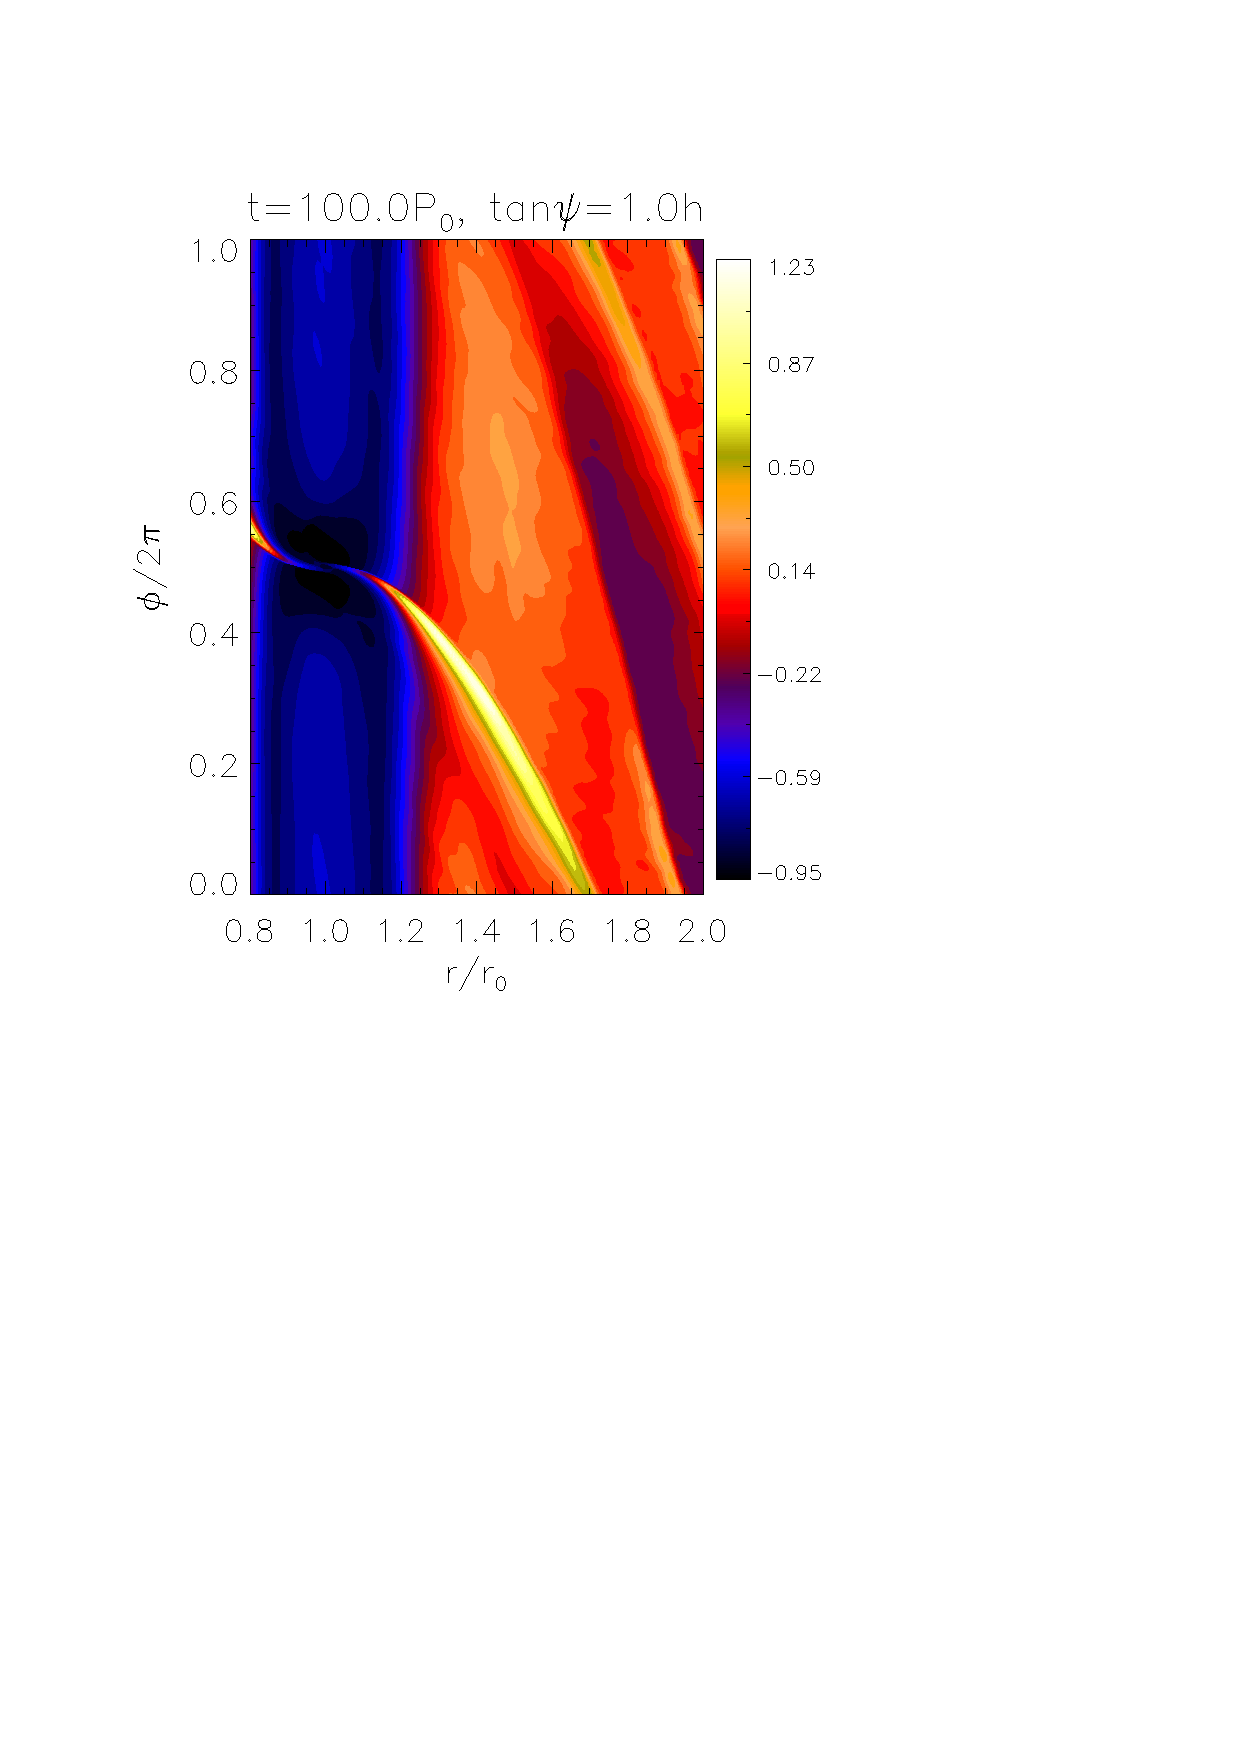
\includegraphics[scale=.39,clip=true,trim=2.3cm
     1.84cm 0cm
     0cm]{figures/jup1_3h_pdisk008}
   \caption{Density perturbation $\delta\rho$ at the end of the
     disc-planet simulations case P3 (left, no viscous layer) and P4
     (right, viscous layer occupies $33\%$ of the uppermost vertical
     domain).   
     \label{jup0_3h}}
\end{figure}
 


